\documentclass[oneside]{amsart}
\linespread{2}
%
% This document is a preamble for 'reopn' project
%

% ==============================
% Load Packages
% ==============================

\usepackage{amsfonts}
\usepackage{amssymb}  
\usepackage{amsthm} 
\usepackage{amsmath} 
\usepackage{caption}
\usepackage[inline]{enumitem}
  \setlist{itemsep=0em, topsep=0em, parsep=0em}
  \setlist[enumerate]{label=(\alph*)}
\usepackage{etoolbox}
\usepackage{stmaryrd} 
\usepackage[dvipsnames]{xcolor}
  \definecolor{myurlcolor}{rgb}{0.6,0,0}
  \definecolor{mycitecolor}{rgb}{0,0,0.8}
  \definecolor{myrefcolor}{rgb}{0,0,0.8}
\usepackage[pagebackref]{hyperref}
\usepackage{hyperref}
\hypersetup{colorlinks,
	linkcolor=myrefcolor,
	citecolor=mycitecolor,
	urlcolor=myurlcolor}
\usepackage{graphicx}
  \graphicspath{ {assets/} }
\usepackage{mathtools}
\usepackage{tikz}
  \usetikzlibrary{matrix,
    arrows,
    shapes,
    decorations.markings,
    decorations.pathreplacing}
\usepackage{todonotes}

% ====================================
% New Commands
% ====================================

\renewcommand*{\backref}[1]{(Referred to on page #1.)}

% symbols ~~~~~~~~~~~~~~~~~~~~~~~~~~~
\renewcommand{\epsilon}{\varepsilon}
\newcommand{\op}{^{\scriptsize{ \textrm{op} } }}
\newcommand{\inv}{^{-1}}
\newcommand{\iso}{\cong}
\renewcommand{\equiv}{\simeq}
\newcommand{\bydef}{\coloneqq}
\newcommand{\hcirc}{\circ_{\textup{h}}}
\newcommand{\vcirc}{\circ_{\textup{v}}}
\renewcommand{\hat}{\widehat}


% categories ~~~~~~~~~~~~~~~~~~~~~~~~~
\newcommand{\A}{\cat{A}}
\newcommand{\B}{\cat{B}}
\newcommand{\C}{\cat{C}}
\newcommand{\D}{\cat{D}}
\newcommand{\E}{\cat{E}}
\renewcommand{\P}{\cat{P}}
\newcommand{\Q}{\cat{Q}}
\newcommand{\R}{\cat{R}}
\newcommand{\T}{\cat{T}}
\newcommand{\U}{\cat{U}}
\newcommand{\V}{\cat{V}}
\newcommand{\W}{\cat{W}}
\newcommand{\X}{\cat{X}}
\newcommand{\Y}{\cat{Y}}
\newcommand{\Z}{\cat{Z}}
\renewcommand{\AA}{\bicat{A}}
\newcommand{\BB}{\bicat{B}}
\newcommand{\CC}{\bicat{C}}
\newcommand{\DD}{\bicat{D}}
\newcommand{\EE}{\bicat{E}}
\newcommand{\PP}{\bicat{P}}
\newcommand{\QQ}{\bicat{Q}}
\newcommand{\RR}{\bicat{R}}
\newcommand{\TT}{\bicat{T}}
\newcommand{\UU}{\bicat{U}}
\newcommand{\VV}{\bicat{V}}
\newcommand{\WW}{\bicat{W}}
\newcommand{\XX}{\bicat{X}}
\newcommand{\YY}{\bicat{Y}}
\newcommand{\ZZ}{\bicat{Z}}
\newcommand{\AAA}{\dblcat{A}}
\newcommand{\BBB}{\dblcat{B}}
\newcommand{\CCC}{\dblcat{C}}
\newcommand{\DDD}{\dblcat{D}}
\newcommand{\EEE}{\dblcat{E}}
\newcommand{\MMM}{\dblecat{M}}
\newcommand{\PPP}{\dblcat{P}}
\newcommand{\QQQ}{\dblcat{Q}}
\newcommand{\RRR}{\dblcat{R}}
\newcommand{\SSS}{\dblcat{S}}
\newcommand{\TTT}{\dblcat{T}}
\newcommand{\UUU}{\dblcat{U}}
\newcommand{\VVV}{\dblcat{V}}
\newcommand{\WWW}{\dblcat{W}}
\newcommand{\XXX}{\dblcat{X}}
\newcommand{\YYY}{\dblcat{Y}}
\newcommand{\ZZZ}{\dblcat{Z}}

% common x-categories
\newcommand{\FinSet}{\cat{FinSet}}
\newcommand{\Set}{\cat{Set}}
\newcommand{\Rel}{\cat{Rel}}
\newcommand{\RRel}{\bicat{Rel}}
\newcommand{\FinHilb}{\cat{FinHilb}}
\newcommand{\Ab}{\cat{Ab}}
\newcommand{\Vect}{\cat{Vect}}
\newcommand{\Mod}{\cat{Mod}}
\newcommand{\Pos}{\cat{Pos}}
\newcommand{\FinGraph}{\cat{FinGraph}}
\newcommand{\Graph}{\cat{Graph}}
\newcommand{\RGraph}{\cat{RGraph}}
\newcommand{\Top}{\cat{Top}}
\newcommand{\TTop}{\bicat{Top}}
\newcommand{\Cat}{\cat{Cat}}
\newcommand{\CCat}{\bicat{Cat}}
\newcommand{\Bicat}{\cat{Bicat}}
\newcommand{\BBicat}{\bicat{Bicat}}
\newcommand{\DblCat}{\cat{DblCat}}
\newcommand{\DDblCat}{\bicat{DblCat}}
\newcommand{\Topos}{\cat{Topos}}
\newcommand{\TTopos}{\bicat{Topos}}
\newcommand{\Span}{\cat{Span}}
\newcommand{\SSpan}{\bicat{Span}}
\newcommand{\Csp}{\cat{Csp}}
\newcommand{\CCsp}{\bicat{Csp}}
\newcommand{\Gram}{\cat{Gram}}
\newcommand{\StrCsp}{\cat{StrCsp}}
\newcommand{\SStrCsp}{\bicat{StrCsp}}
\newcommand{\SSStrCsp}{\dblcat{S} \bicat{trCsp}}
\newcommand{\StrCspGram}{\cat{StrCspGram}}
\newcommand{\RRewrite}{\bicat{Rewrite}}
\newcommand{\RRRewrite}{\dblcat{R}\bicat{ewrite}}
\newcommand{\ZX}{\cat{ZX}}
\newcommand{\ZZX}{\bicat{ZX}}
\newcommand{\ZZZX}{\dblcat{ZX}}
\newcommand{\FinGraphGamma}{\FinGraph \downarrow \Gamma}
\newcommand{\AdjTopos}{\cat{AdjTopos}}

% functors ~~~~~~~~~~~~~~~~~~~~~~~~~
\newcommand{\core}{\mathbf{core}}
\newcommand{\Lang}{\mathrm{Lang}}

% text formatting ~~~~~~~~~~~~~~~~~~~~~
\newcommand{\df}[1]{\textbf{#1}}
\newcommand{\cat}[1]{\mathsf{#1}}
\newcommand{\bicat}[1]{\mathbf{#1}}
\newcommand{\dblcat}[1]{\mathbb{#1}}
\newcommand{\type}[1]{\mathtt{#1}}
\newcommand{\Daniel}[1]{\textcolor{red}{(#1)}}

% arrows ~~~~~~~~~~~~~~~~~~~~~~~~~~~~~~
\newcommand{\from}{\colon}
\newcommand{\rel}{\nrightarrow}
\newcommand{\To}{\Rightarrow}
\newcommand{\xto}[1]{\xrightarrow{#1}}
\newcommand{\monicto}{\rightarrowtail}
\newcommand{\dderiv}[2]{#1 \rightsquigarrow #2}
\newcommand{\deriv}[2]{#1 \rightsquigarrow^\ast #2}
\renewcommand{\gets}{\leftarrow}
\newcommand{\monicgets}{\leftarrowtail}
\newcommand{\xgets}[1]{\xleftarrow{#1}}
\newcommand{\spn}[3]{#1 \gets #2 \to #3}
\newcommand{\xspn}[5]{#1 \xgets{#2} #3 \xto{#4} #5}
\newcommand{\csp}[3]{#1 \to #2 \gets #3}
\newcommand{\xcsp}[5]{#1 \xto{#2} #3 \xgets{#4} #5}
\newcommand{\lrto}{\rightleftarrows}

% math operators ~~~~~~~~~~~~~~~~~~~~~~~~~
\DeclareMathOperator{\Hom}{Hom}
\DeclareMathOperator{\id}{id}
\DeclareMathOperator{\im}{im}
\DeclareMathOperator{\Sub}{Sub}
\DeclareMathOperator{\colim}{colim}
\DeclareMathOperator{\ob}{ob}
\DeclareMathOperator{\arr}{arr}
\DeclareMathOperator{\edges}{edges}
\DeclareMathOperator{\nodes}{nodes}
\DeclareMathOperator{\decat}{decat}

% delimiters ~~~~~~~~~~~~~~~~~~~~~~~~~
%\renewcommand{\l(}{\left(}
%\newcommand{\r)}{\right)}

% =========================================
% Environments and Counters
% =========================================

\newtheorem{theorem}{Theorem}[section]
\newtheorem*{theorem*}{Theorem}
\newtheorem{lemma}[theorem]{Lemma}
\newtheorem{proposition}[theorem]{Proposition}
\newtheorem{corollary}[theorem]{Corollary}

\theoremstyle{remark}
\newtheorem{remark}[theorem]{Remark}
\newtheorem{notation}[theorem]{Notation}

\theoremstyle{definition}
\newtheorem{example}[theorem]{Example} 
\newtheorem{definition}[theorem]{Definition}

\setcounter{tocdepth}{1} % Sets depth for table of contents. 

% ==========================================
% Tikz Macros
% ==========================================

% arrows for commuting diagrams
\tikzset{
  cd/.style={
    ->,
    scale=6,
    >=angle 90,
    font=\scriptsize}}

% arrows for graphs
\tikzset{
  graph/.style={
    ->,
    scale=2,
    >=triangle 45,
    font=\scriptsize}}

% arrow head in middle of edge
\tikzset{->-/.style={decoration={%
      markings,
      mark=at position .5 with {\arrow{>}}},
      postaction={decorate}}}

% arrow head user-positioned
\tikzset{->-pos/.style={decoration={%
      markings,
      mark=at position #1 with {\arrow{>}}},
      postaction={decorate}}}

% arrow head in middle of edge
\tikzset{-|->/.style={decoration={%
      markings,
      mark=at position .5 with {\arrow{|}},
      mark=at position 1 with {\arrow{>}}},
    postaction={decorate}}}

% walking reflexive graph
\newcommand{\rgraph}[2]{%
  \begin{tikzpicture}[scale=0.75,baseline=-3pt]
    \node (a) at (0,0) {$ #1 $};
    \node (b) at (1,0) {$ #2 $};
    \draw [->]
    ([yshift= 4pt]a.east) to ([yshift= 4pt]b.west);
    \draw [->]
    ([yshift=-4pt]a.east) to ([yshift=-4pt]b.west);
    \draw [->]
    (b.west) to (a.east);
  \end{tikzpicture}
}

% walking graph
\newcommand{\graph}[2]{%
  \begin{tikzpicture}[scale=0.75,baseline=-3pt]
    \node (a) at (0,0) {$ #1 $};
    \node (b) at (1,0) {$ #2 $};
    \draw [->]
    ([yshift=4pt]a.east) to ([yshift=4pt]b.west);
    \draw [->]
    ([yshift=-4pt]a.east) to ([yshift=-4pt]b.west);
  \end{tikzpicture}
}

% open tipped arrow
\newcommand{\opento}[2]{%
  \begin{tikzpicture}[scale=0.75,baseline=-3pt]
    \node (a) at (0,0) {$ #1 $};
    \node (b) at (1,0) {$ #2 $};
    \draw [->, open triangle 60]
    (a.east) to (b.west);
  \end{tikzpicture}
}

% inline horizontal arrow
\newlength\mylen
\settowidth\mylen{$\to$}

\newcommand{\horarrow}{%
  \to\kern-0.55\mylen\vline height 1.2ex depth
  -0.4pt\kern0.55\mylen}

% adjunction
\newcommand{\adjunction}[4]{%
  \begin{tikzpicture}[baseline=-3pt]
    \node (1) at (0,0) {\( #1 \)};
    \node (2) at (2,0) {\( #4 \)};
    \draw [->]
    ([yshift= 4pt]2.west) to
    node [above] {\scriptsize{ $ #2 $ }}
    ([yshift= 4pt]1.east);
    \draw [->]
    ([yshift= -4pt]1.east) to
    node [below] {\scriptsize{ $ #3 $ }}
    node [above,yshift= -1.5pt] {\scriptsize{$ \perp $}}
    ([yshift= -4pt]2.west);
  \end{tikzpicture}
  % 
}

\begin{document}
\author{Daniel Cicala}
\title{Rewriting structured cospans}
\date{\today}
\email{dcicala@newhaven.edu}
\address{Department of Mathematics and Physics\\
  University of New Haven}
\maketitle

\begin{abstract}
  To foster the study of networks on an abstract level, we
  further study the formalism of \emph{structured cospans}
  introduced by Baez and Courser. A structured cospan is a
  diagram of the form $ La \to x \gets Lb $ built from a
  geometric morphism with left exact left adjoint
  $ L \dashv R \from \X \to \A $.  We show that this
  construction is functorial and results in a topos with
  structured cospans for objects.  Additionally, structured
  cospans themselves are compositional. Combining these two
  perspectives, we define a double category of structured
  cospans.  We then leverage adhesive categories to create a
  theory of rewriting for structured cospans. We generalize
  the result from graph rewriting stating that a graph
  grammar induces the same rewrite relation as its
  underlying graph grammar.  We use this fact to prove our
  main result, a complete characterization of the rewriting
  relation for a topos $ \X $ using double categories.  This
  provides a compositional framework for rewriting systems.
\end{abstract}




%% ===================================
%% Introduction
%% ===================================
\section{Introduction}
\label{sec:Intro}

Structured cospans are a framework for reasoning
about systems with inputs and outputs. Rewriting
is a topic that covers methods for editing
substructures of an object such as a string or a
graph. In this paper, we introduce rewriting to
structured cospans.

While the term ``system'' used above is
intentionally vague, a first approximation of what
we have in mind is a collection of discrete
objects that are somehow related. Examples include
home electrical systems consisting of appliances
connected by wires; social systems where people
are connected by social relationships; or virtual
systems such as a collection of webpages connected
by links. These systems are often analyzed as
though they are isolated, that they are
\emph{closed systems}. Indeed, one considers a
single home, or a particular clique of people, or
a single webpage, entirely ignoring that each of
these are actually part of a larger system. A home
lives in power grid, a clique is a merely one
portion of the human population, and a webpage is
actually housed in the internet. That is, these
are really \emph{open systems} that can interact
with the other compatible systems. Structured
cospans offer a way to equip closed systems with
the mechanisms through which these interactions
can occur.

The following toy example suggests a way to fit a system
into its larger context. Suppose we want to analyze the
structure of Professor Smith's academic website, which
contains a home page and two sections. The section devoted
to research comprises, say, five pages connected by several
links as modeled by the graph
\[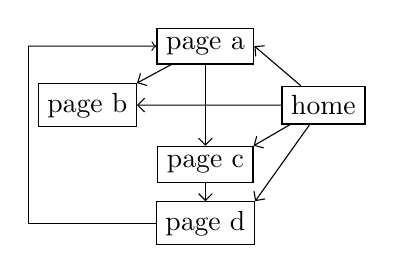
\begin{tikzpicture}[scale=0.75]
    \node[rectangle,draw] (a) at (0,3) {page a};
    \node[rectangle,draw] (b) at (-2,2) {page b};
    \node[rectangle,draw] (h) at (2,2) {home};
    \node[rectangle,draw] (c) at (0,1) {page c};
    \node[rectangle,draw] (d) at (0,0) {page d};
    % 
    \draw [cd]
    (h) edge[] (a.east)
    (h) edge[] (b)
    (h) edge[] (c.north east)
    (h) edge[] (d.north east)
    (a) edge[] (b.north east)
    (a) edge[] (c)
    (c) edge[] (d);
    \draw (d.west) -- (-3,0) -- (-3,3);
    \draw [->] (-3,3) to (a.west); 
  \end{tikzpicture}\] The section devoted to
teaching comprises, say, three pages connected by several
links as modeled by the graph
\[
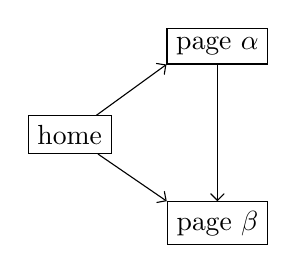
\begin{tikzpicture}[scale=0.75]  
  \node[rectangle,draw] (h) at (-0.5,1.5) {home};
  \node[rectangle,draw] (a) at (2,3) {page $\alpha$};
  \node[rectangle,draw] (b) at (2,0) {page $\beta$};
  %
  \draw [cd]
  (h) edge[] (a.south west)
  (h) edge[] (b.north west)
  (a) edge[] (b);  
\end{tikzpicture}
\] These graphical models
are amenable to analysis using tools from network
theory. However, such graphical models fail to capture that
Professor Smith's website is part of the larger internet,
rather, that it is an open system. This leads to us
replacing each graph in our model with an \emph{open graph},
meaning a graph equipped with two sets of nodes interpreted
as `inputs' and `outputs' (terms not meant to imply
causality). We can promote a graph to an open graph by
equipping it with a pair of functions from discrete graphs
that effectively select the inputs and outputs. For instance
\begin{equation} \label{eq:Intro_OpenGraph1}
  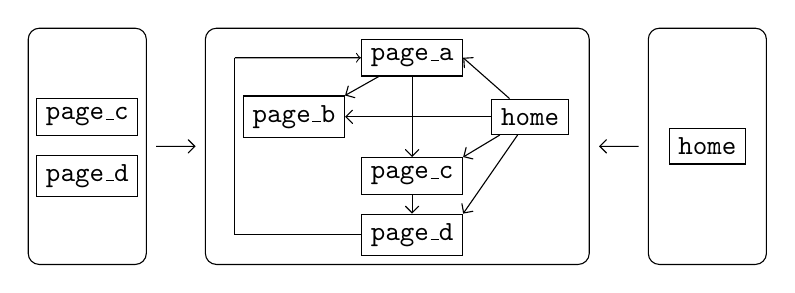
\begin{tikzpicture}[
    scale=0.75,
    baseline=(current bounding box.center)]
    \begin{scope}[shift={(-5.5,0)}]
      \node[rectangle,draw] (1) at (0,2) {$\mathtt{page\_c}$};
      \node[rectangle,draw] (1) at (0,1) {$\mathtt{page\_d}$};
      \draw [rounded corners] (-1,-0.5) rectangle (1,3.5);
      \node (indom) at (1,1.5) {};
    \end{scope}
    \begin{scope}
      \node[rectangle,draw] (a) at (0,3) {$\mathtt{page\_a}$};
      \node[rectangle,draw] (b) at (-2,2) {$\mathtt{page\_b}$};
      \node[rectangle,draw] (h) at (2,2) {$\mathtt{home}$};
      \node[rectangle,draw] (c) at (0,1) {$\mathtt{page\_c}$};
      \node[rectangle,draw] (d) at (0,0) {$\mathtt{page\_d}$};
      % 
      \draw [cd]
      (h) edge[] (a.east)
      (h) edge[] (b)
      (h) edge[] (c.north east)
      (h) edge[] (d.north east)
      (a) edge[] (b.north east)
      (a) edge[] (c)
      (c) edge[] (d);
      \draw (d.west) -- (-3,0) -- (-3,3);
      \draw [->] (-3,3) to (a.west);
      \draw [rounded corners] (-3.5,-0.5) rectangle (3,3.5);
      \node (incod) at (-3.5,1.5) {};
      \node (outcod) at (3,1.5) {};
    \end{scope}
    \begin{scope}[shift={(5,0)}]
      \node [rectangle,draw] (1) at (0,1.5) {$\mathtt{home}$};
      \draw [rounded corners] (-1,-0.5) rectangle (1,3.5); 
      \node (outdom) at (-1,1.5) {};    
    \end{scope}    
    %
    \draw [cd]
    (indom) edge (incod)
    (outdom) edge (outcod);
\end{tikzpicture}
\end{equation}
 endows the graph with
input nodes \texttt{page b} and \texttt{page c} and output
nodes \texttt{home}. Likewise
\begin{equation} \label{eq:Intro_OpenGraph2}
  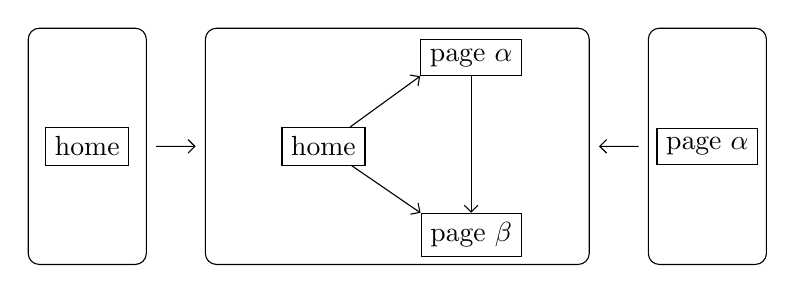
\begin{tikzpicture}[
    scale=0.75,
    baseline=(current bounding box.center)]
    \begin{scope}[shift={(-5.5,0)}]
      \node [rectangle,draw] (1) at (0,1.5) {home};
      \draw [rounded corners] (-1,-0.5) rectangle (1,3.5); 
      \node (indom) at (1,1.5) {};
    \end{scope}
    \begin{scope}
      \node[rectangle,draw] (h) at (-1.5,1.5) {home};
      \node[rectangle,draw] (a) at (1,3) {page $\alpha$};
      \node[rectangle,draw] (b) at (1,0) {page $\beta$};
      % 
      \draw [cd]
      (h) edge[] (a.south west)
      (h) edge[] (b.north west)
      (a) edge[] (b);
      \draw [rounded corners] (-3.5,-0.5) rectangle (3,3.5);
      \node (incod) at (-3.5,1.5) {};
      \node (outcod) at (3,1.5) {};
    \end{scope}  
    \begin{scope}[shift={(5,0)}]
      \node [rectangle,draw] (1) at (0,1.5) {page $\alpha$};
      \draw [rounded corners] (-1,-0.5) rectangle (1,3.5);
      \node (outdom) at (-1,1.5) {};
    \end{scope}
    % 
    \draw [cd]
    (indom) edge (incod)
    (outdom) edge (outcod);
\end{tikzpicture}
\end{equation} endows the graph with
input nodes \texttt{home} and output nodes \texttt{page\_e}.
These cospans provide a mechanism to connect compatible
systems together, thus allowing us to see how a system fits
into its surroundings. Observe that the outputs of
\eqref{eq:Intro_OpenGraph1} match the inputs of
\eqref{eq:Intro_OpenGraph2}. This indicates that the two
sections of the website share a page, namely the home page.
It also means that we can model the entire website by
connecting the two graphs along that common node
\[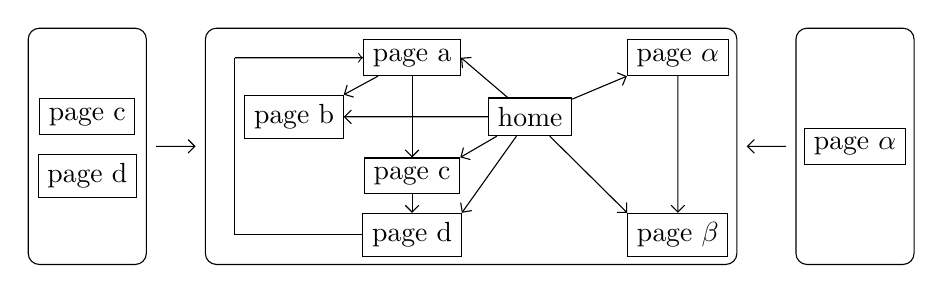
\begin{tikzpicture}[scale=0.75]
    \begin{scope}[shift={(-5.5,0)}]
      \node[rectangle,draw] (1) at (0,2) {page c};
      \node[rectangle,draw] (1) at (0,1) {page d};
      \draw [rounded corners] (-1,-0.5) rectangle (1,3.5);
      \node (indom) at (1,1.5) {};
    \end{scope}
    \begin{scope}
      \node[rectangle,draw] (a) at (0,3) {page a};
      \node[rectangle,draw] (b) at (-2,2) {page b};
      \node[rectangle,draw] (h) at (2,2) {home};
      \node[rectangle,draw] (c) at (0,1) {page c};
      \node[rectangle,draw] (d) at (0,0) {page d};
      \node[rectangle,draw] (a') at (4.5,3) {page $\alpha$};
      \node[rectangle,draw] (b') at (4.5,0) {page $\beta$};
      %      
      \draw [cd]
      (h) edge[] (a.east)
      (h) edge[] (b)
      (h) edge[] (c.north east)
      (h) edge[] (d.north east)
      (a) edge[] (b.north east)
      (a) edge[] (c)
      (c) edge[] (d);
      \draw (d.west) -- (-3,0) -- (-3,3);
      \draw [->] (-3,3) to (a.west);
      % 
      \draw [cd]
      (h) edge[] (a'.south west)
      (h) edge[] (b'.north west)
      (a') edge[] (b');
      %      
      \draw [rounded corners] (-3.5,-0.5) rectangle (5.5,3.5);
      \node (incod) at (-3.5,1.5) {};
      \node (outcod) at (5.5,1.5) {};
    \end{scope}
    \begin{scope}[shift={(7.5,0)}]
      \node [rectangle,draw] (1) at (0,1.5) {page $ \alpha $};
      \draw [rounded corners] (-1,-0.5) rectangle (1,3.5); 
      \node (outdom) at (-1,1.5) {};    
    \end{scope}    
    %
    \draw [cd]
    (indom) edge (incod)
    (outdom) edge (outcod);
\end{tikzpicture}\] This example can be
formalized using structured cospans.

Baez and Courser introduced structured cospans as
an abstract framework to model open systems
\parencite{bc_strCsp}. A structured cospan is a diagram
of the form
\begin{equation}\label{eq:Intro_StrCspForm}
  La \to x \gets Lb
\end{equation}
where $ L \from \A \to \X $ is a functor whose
codomain $ \X $ has pushouts. This functor is a
nice bookkeeping device that allows us to separate
the system types into $ \X $ and the interface
types into $ \A $.  We then interpret
\eqref{eq:Intro_StrCspForm} as a system $ x $ with
inputs $ La $ and outputs $ Lb $. There is a
category $ _L\Csp $ whose objects are those of
$ \A $ and arrows are (isomorphism classes of) structured cospans
$ La \to x \gets Lb $ that compose by pushout:
$$(La \to x \gets Lb \to y \gets Lc) \mapsto (La \to x +_{Lb}y
\gets Lc)$$ In the example above,
$ \A \bydef \Set $, $ \X \bydef \Graph $, and
$ L $ turns a set into a discrete graph.

Given the ability to model open systems using
structured cospans, we would like tools to analyze
these models. In this paper, we adapt for
structured cospans the tool of double pushout
(DPO) rewriting, an algorithmic technique for
creating a new object from an old object according
to some given set of rules. One application of
rewriting is to `simplify' objects. For example,
in the case of electrical circuits, rewriting
provides a method to replace an instance of
\[\begin{circuitikz}[scale=0.75]
    \draw (0,0)
    to[R=$ R_1 $] (2,0)
    to[short] (3,0)
    to[R=$ R_2 $] (5,0);
  \end{circuitikz}\] in a circuit
diagram with \[\begin{circuitikz}[scale=0.75]
  \draw (0,0)
  to[R=$\mathtt{R}_1+\mathtt{R}_2$] (2,0);
\end{circuitikz}\]

Rewriting works nicely in any adhesive category
\parencite{LackSobo_Adhesive}. However, we restrict our
attention to a specific type to adhesive category
called a topos \parencite{LackSobo_TopsIsAdh}. The
reasons for this are both technical (we eventually
required Cartesian closedness) and promotional
(topoi are more widely known and are more easily
understood than adhesive categories).

In DPO rewriting, one starts with a \emph{grammar}
$ ( \T,P ) $, that is an topos $ \T $ and a set
$ P \bydef \{ \ell_j \gets k_j \to r_j \} $ of spans in $ \T $ with monic arrows. These
spans are called \emph{rules}. We interpret a rule
$ \ell \gets k \to r $ as stating that $ r $
replaces $ \ell $ in a manner that fixes $ k
$. This rule can be applied to any object
$ \ell' $ by realizing a \emph{double pushout
  diagram} \begin{equation} \label{eq:Intro_DpoDiagram}
  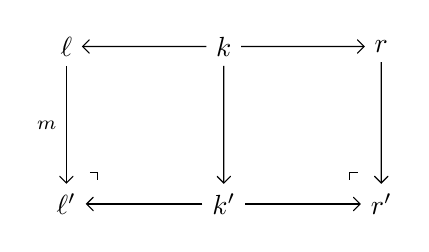
\begin{tikzpicture}[
    baseline=(current bounding box.center)]
    scale=0.75]
    \node (1) at (0,2) {$ \ell $};
    \node (2) at (2,2) {$ k $};
    \node (3) at (4,2) {$ r $};
    \node (4) at (0,0) {$ \ell' $};
    \node (5) at (2,0) {$ k' $};
    \node (6) at (4,0) {$ r' $};
    \draw [cd]
    (2) edge (1)
    (2) edge (3)
    (5) edge (4)
    (5) edge (6)
    (1) edge node[left]{$ m $} (4)
    (2) edge (5)
    (3) edge (6); 
    \draw (0.3,0.4) -- (0.4,0.4) -- (0.4,0.3);
    \draw (3.7,0.4) -- (3.6,0.4) -- (3.6,0.3);
  \end{tikzpicture}
\end{equation}

where $ m $ identifies an instance of $ \ell $ in
$ \ell' $ and that instance is then replaced by
$ r $, thus resulting in the new object $ r'
$. The squares being pushouts ensure that the
glueing condition is met, which in the case of
graphs, means that there are no nodes removed
that leave an edge unanchored.

To study a grammar $ ( \T , P ) $, one studies its
rewrite relation. Assuming that $ P $ contains the
rule $ \ell \gets k \to r $, the span across the
bottom of \eqref{eq:Intro_DpoDiagram} is called a
\emph{derived rule}. Collecting all derived rules
$ \ell' \gets k' \to r' $ associated to
$ ( \T,P ) $, we define a relation
$ \ell' \rightsquigarrow r' $.  The reflexive and
transitive closure $ \rightsquigarrow^\ast $ is called
the \emph{rewrite relation} for $ ( \T,P ) $.  The
meaning of $ x \rightsquigarrow^\ast y $ is that
there is a finite sequence of rules in $ P $ through
which $ x $ can be rewritten into $ y $.  In some
sense, $ y $ is a simplification of $ x $. From
$ ( \T,P ) $ and its associated rewrite relation,
we can build a category $ \Lang ( \T,P ) $ called
the \emph{language} of $ (\T,P) $. Often, the
terms ``language'' and ``rewrite relation'' are
used interchangeably, but we will reserve the
former for the category theoretical perspective
and the latter for the relational perspective.
The category $ \Lang (\T,P) $ has the same objects
as $ \T $ and the arrows $ x \to y $ witness
$ x \rightsquigarrow^\ast y $. In fact, by
defining a category $ \Gram $ of grammars,
$ \Lang $ is seen to be functorial
$ \Lang \from \Gram \to \Cat $ (Theorem
\ref{thm:Lang_from_Gram_to_Cat}) thus encoding the
rewrite relation in a category.

In order to bring structured cospans into the
theory of rewriting, we show that they form a
topos. This is true under certain conditions.
Define a category $ _L\StrCsp $ whose objects are
structured cospans and arrows are commuting
diagrams \[
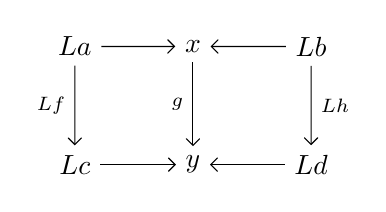
\begin{tikzpicture}[scale=0.75]
  \node (1) at (-2,2) {\( La \)};
  \node (2) at (0,2) {\( x \)};
  \node (3) at (2,2) {\( Lb \)};
  \node (4) at (-2,0) {\( Lc \)};
  \node (5) at (0,0) {\( y \)};
  \node (6) at (2,0) {\( Ld \)};
  \draw [cd]
    (1) edge node[]{} (2)
    (3) edge node[]{} (2)
    (4) edge node[]{} (5)
    (6) edge node[]{} (5)
    (1) edge node[left]{$Lf$}  (4)
    (2) edge node[left]{$g$}   (5)
    (3) edge node[right]{$Lh$} (6);
\end{tikzpicture}
\] If $ L $
is a geometric morphism, that is a left exact left
adjoint between topoi, then $ _L\StrCsp $ is a topos because is
it equivalent to the Artin glueing
$ \A \times \A \downarrow \Delta R $ where $ R $
is right adjoint to $ L $ and
$ \Delta \from \A \to \A \times \A $ is the
diagonal functor (Theorem \ref{thm:strcsp-istopos}).

Even though we are restricting $ L $ more than
Baez and Courser, our definition still covers many
important examples.  One such example is the
discrete graph functor $ L \from \Set \to \Graph $
mentioned above. More examples come by using slice
categories $ \Graph / g $ for some graph $ g $
chosen to endow nodes and arrows with types as was
done to model the ZX-calculus \parencite{ZX}.

Because $ _L\StrCsp $ is a topos, it supports a
rich theory of rewriting. An analysis begins with
a \emph{structured cospan grammar}
$ (_L\StrCsp, P) $, which is different than a
grammar as discussed above because we require
$ P $ to contain spans in $ _L\StrCsp $ of the
form \[
  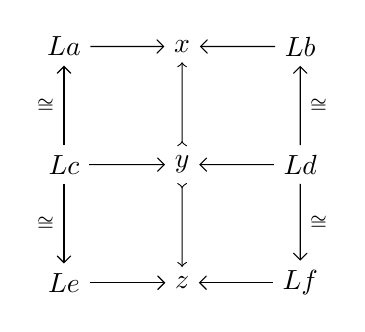
\begin{tikzpicture}[
    baseline=(current bounding box.center),
    scale=0.75]
    \node (a) at (0,4) {$ La $};
    \node (b) at (2,4) {$ x $};
    \node (c) at (4,4) {$ Lb $};
    \node (x) at (0,2) {$ Lc $};
    \node (y) at (2,2) {$ y $};
    \node (z) at (4,2) {$ Ld $};
    \node (d) at (0,0) {$ Le $};
    \node (e) at (2,0) {$ z$};
    \node (f) at (4,0) {$ Lf $};
    %    
    \draw [>->] (y) to (b);
    \draw [>->] (y) to (e);
    \draw[cd]
    (a) edge[] (b)
    (x) edge[] (y)
    (d) edge[] (e)
    (c) edge[] (b)
    (z) edge[] (y)
    (f) edge[] (e)
    (x) edge[] node[left]{$ \iso $}  (a)
    (z) edge[] node[right]{$ \iso $} (c)
    (x) edge[] node[left]{$ \iso $}  (d)
    (z) edge[] node[right]{$ \iso $} (f) ;
  \end{tikzpicture}
\]
 This condition
is stronger than simply requiring monic-legged
spans due to the isomorphisms present. These
isomorphisms ensure that rewriting cannot change
the interface of a system. 

Given a structured cospan grammar, we can
construct its language in a functorial way.  This
starts with an observation: there are two
compositional structures at play. There is the
compositionality of the rules, seen by placing two
atop one another
\[
  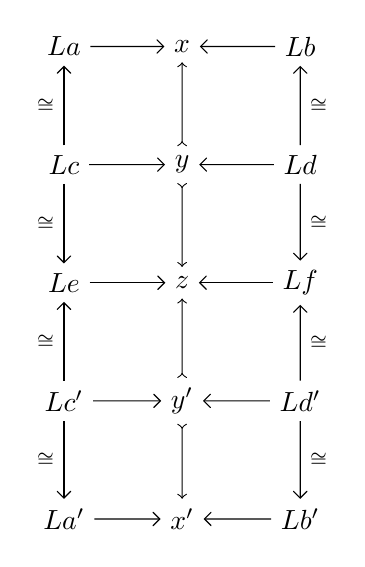
\begin{tikzpicture}[scale=0.75]
    \node (a) at (0,4) {$ La $};
    \node (b) at (2,4) {$ x $};
    \node (c) at (4,4) {$ Lb $};
    \node (x) at (0,2) {$ Lc $};
    \node (y) at (2,2) {$ y $};
    \node (z) at (4,2) {$ Ld $};
    \node (d) at (0,0) {$ Le $};
    \node (e) at (2,0) {$ z$};
    \node (f) at (4,0) {$ Lf $};
    %
    \node (c') at (0,-2) {$ Lc' $};
    \node (y') at (2,-2) {$ y' $};
    \node (d') at (4,-2) {$ Ld' $};
    \node (a') at (0,-4) {$ La' $};
    \node (x') at (2,-4) {$ x' $};
    \node (b') at (4,-4) {$ Lb' $};
    %    
    \draw [>->] (y) to (b);
    \draw [>->] (y) to (e);
    \draw[cd]
    (a) edge[] (b)
    (x) edge[] (y)
    (d) edge[] (e)
    (c) edge[] (b)
    (z) edge[] (y)
    (f) edge[] (e)
    (x) edge[] node[left]{$ \iso $}  (a)
    (z) edge[] node[right]{$ \iso $} (c)
    (x) edge[] node[left]{$ \iso $}  (d)
    (z) edge[] node[right]{$ \iso $} (f) ;
    %
    \draw [cd]
    (c') edge node[]{$  $} (y')
    (d') edge node[]{$  $} (y')
    (a') edge node[]{$  $} (x')
    (b') edge node[]{$  $} (x')
    (c') edge node[left]{$ \iso $} (d)
    (d') edge node[right]{$ \iso $} (f)
    (c') edge node[left]{$ \iso $} (a')
    (d') edge node[right]{$ \iso $} (b');
    \draw [>->] (y') to (e);
    \draw [>->] (y') to (x');
  \end{tikzpicture}
  \] and obtaining
the composite \[
  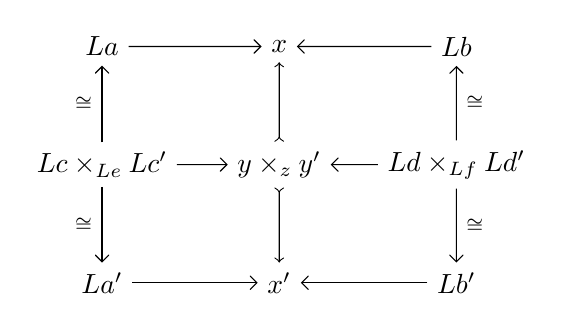
\begin{tikzpicture}[scale=0.75]
    \node (a) at (0,4) {$ La $};
    \node (b) at (3,4) {$ x $};
    \node (c) at (6,4) {$ Lb $};
    \node (x) at (0,2) {$ Lc \times_{Le} Lc'  $};
    \node (y) at (3,2) {$ y \times_{z} y' $};
    \node (z) at (6,2) {$ Ld \times_{Lf} Ld' $};
    \node (d) at (0,0) {$ La' $};
    \node (e) at (3,0) {$ x'$};
    \node (f) at (6,0) {$ Lb' $};
    %    
    \draw [>->] (y) to (b);
    \draw [>->] (y) to (e);
    \draw[cd]
    (a) edge[] (b)
    (x) edge[] (y)
    (d) edge[] (e)
    (c) edge[] (b)
    (z) edge[] (y)
    (f) edge[] (e)
    (x) edge[] node[left]{$ \iso $}  (a)
    (z) edge[] node[right]{$ \iso $} (c)
    (x) edge[] node[left]{$ \iso $}  (d)
    (z) edge[] node[right]{$ \iso $} (f) ;
    %
  \end{tikzpicture}
  \]
using pullback. In classical rewriting, this
is the only composition.  New to structured cospan
rewriting is the compositionality of the
structured cospans themselves, seen by placing
rules beside one another
\[
    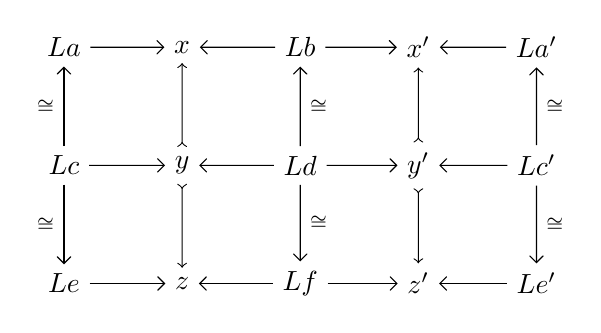
\begin{tikzpicture}[scale=0.75]
    \node (a) at (0,4) {$ La $};
    \node (b) at (2,4) {$ x $};
    \node (c) at (4,4) {$ Lb $};
    \node (x) at (0,2) {$ Lc $};
    \node (y) at (2,2) {$ y $};
    \node (z) at (4,2) {$ Ld $};
    \node (d) at (0,0) {$ Le $};
    \node (e) at (2,0) {$ z$};
    \node (f) at (4,0) {$ Lf $};
    %
    \node (x') at (6,4) {$ x' $};
    \node (y') at (6,2) {$ y' $};
    \node (z') at (6,0) {$ z' $};
    \node (a') at (8,4) {$ La' $};
    \node (c') at (8,2) {$ Lc' $};
    \node (e') at (8,0) {$ Le' $};
    %    
    \draw [>->] (y) to (b);
    \draw [>->] (y) to (e);
    \draw[cd]
    (a) edge[] (b)
    (x) edge[] (y)
    (d) edge[] (e)
    (c) edge[] (b)
    (z) edge[] (y)
    (f) edge[] (e)
    (x) edge[] node[left]{$ \iso $}  (a)
    (z) edge[] node[right]{$ \iso $} (c)
    (x) edge[] node[left]{$ \iso $}  (d)
    (z) edge[] node[right]{$ \iso $} (f) ;
    %
    \draw [cd]
    (c) edge node[]{$  $} (x')
    (z) edge node[]{$  $} (y')
    (f) edge node[]{$  $} (z')
    (a') edge node[]{$  $} (x')
    (c') edge node[]{$  $} (y')
    (e') edge node[]{$  $} (z')
    (c') edge node[right]{$ \iso $} (a')
    (c') edge node[right]{$ \iso  $} (e');
    \draw [>->] (y') to (x');
    \draw [>->] (y') to (z');
  \end{tikzpicture}
  \] and composing
using pushouts \[
    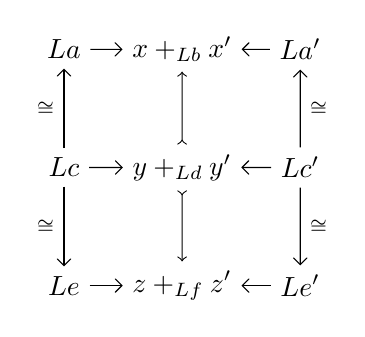
\begin{tikzpicture}[scale=0.75]
    \node (a) at (0,4) {$ La $};
    \node (b) at (2,4) {$ x+_{Lb}x' $};
    \node (c) at (4,4) {$ La' $};
    \node (x) at (0,2) {$ Lc $};
    \node (y) at (2,2) {$ y +_{Ld} y' $};
    \node (z) at (4,2) {$ Lc' $};
    \node (d) at (0,0) {$ Le $};
    \node (e) at (2,0) {$ z +_{Lf} z'$};
    \node (f) at (4,0) {$ Le' $};
    %    
    \draw [>->] (y) to (b);
    \draw [>->] (y) to (e);
    \draw[cd]
    (a) edge[] (b)
    (x) edge[] (y)
    (d) edge[] (e)
    (c) edge[] (b)
    (z) edge[] (y)
    (f) edge[] (e)
    (x) edge[] node[left]{$ \iso $}  (a)
    (z) edge[] node[right]{$ \iso $} (c)
    (x) edge[] node[left]{$ \iso $}  (d)
    (z) edge[] node[right]{$ \iso $} (f) ;
    %
  \end{tikzpicture}
  \]
Because there are two compositional structures,
encoding the language of a structured cospan
grammar into just a category is insufficient.
Evidently, we should instead use a double
category.

The language functor for structured cospans has
type
$$ \Lang \from \StrCspGram \to \DblCat $$ where the
domain is a category whose objects are structured
cospan grammars and codomain is the category of
double categories (Theorem
\ref{thm:StrCsp_Lang_functorial}). Through this
functor, we assign to each structured cospan
grammar $ ( _L\StrCsp,P ) $ a double category
$ \Lang (_L\StrCsp, P) $ serving as its
language. The horizontal arrows of this language
are structured cospans.  The squares are generated
by the rules derived from $ P $. Manifestly, if
one structured cospan can be rewritten into
another using rules in $ P $ then there is a
square between them.  In this sense,
$ \Lang (_L\StrCsp , P) $ encodes the rewrite
relation $ \rightsquigarrow^\ast $.  Although,
there is a new manner of deriving rules through
the compositionality of the structured cospans.
And so, a theory of rewriting is established.

Further work is required to study properties of
the languages arising from structured cospan
grammars. Now, we turn our attention to an
application of rewriting structured cospans.

In the classical topics of rewriting, formal
languages and term rewriting, there are two
approaches to defining the rewrite relation for a
grammar. The first is an operational definition
which stipulates when a rule can be applied by
using sub-terms and substitution.  The other is an
inductive definition which constructs the rewrite
relation using generators and closure
operations. When rewriting theory expanded to
graphs in the 1970's, only the operational
definition prevailed.  Then in the 1990's, Gadducci
and Heckel introduced an inductive definition to
graph rewriting
\parencite{Gadd_IndGraphTrans}, thus allowing for
analyses using structural induction. With the new
technology of structured cospans, we can use their
ideas to bring the inductive viewpoint to
rewriting in a large class of topoi.

A central idea in developing the inductive
definition is to equip graphs with an
interface. Earlier, we referred to such graphs as
open, but Gadducci and Heckel called them ``ranked
graphs''.  To bring this idea to objects of a
topos, we can use structured cospans. That is, if
$ \X $ is a topos that fits into a geometric
morphism $ L \dashv R \from \X \to \A $ with a
monic counit, then an \emph{object $ x $ with an
interface} is a structured cospan $ La \to x \gets
Lb$. The induced comonad on $ \X $ can be though
of as returning the maximal, with respect to
inclusion, interface $ LRx $ of each object $ x
$. The monic counit $ LRx \to x $ simply includes
that interface.

Another pillar in the construction of the inductive
definition is the equivalence between two classes of rewrite
relations.  In the context of graph rewriting, this result
states that the rewrite relation for a graph grammar
$$(\Graph , \{ \ell_j \gets k_j \to r_j\})$$ is the same as for the `discrete graph
grammar'
$$( \Graph , \{ \ell_j \gets k'_j \to r_j\})$$ where $ k'_j $ is the discrete graph
underlying $ k_j $ and the arrows in the rules of the latter
grammar are obtained by restriction the arrows of
the former.  To extend this to rewriting in a topos, we
again use a comonad $ LR $ induced from a geometric morphism
with a monic counit. It allows us to access the `discrete'
objects $ LRx $ underlying an arbitrary object $ x $.  In
the generalized setting, the rewrite relation for the
grammar $ ( \X, \{ \ell_j \gets k_j \to r_j\}) $ is the same
as for the grammar
$ (\X , \{ \ell_j \gets LR k_j \to r_j\}) $ as long as the
subobject lattices $ \Sub (k_j) $ have all meets (Theorem
\ref{thm:production-same-rewrite-relation-as-discrete}).

We now have the ability to equip the objects of a
topos with an interface using structured cospans
and we have established that a grammar and its
`discretized' version induce the same rewrite relation.
Next, we can provide an inductive definition for
the language. Fix a grammar
$ (\X, \{ \ell_j \gets k_j \to r_j\}) $
such that $ \X $ fits into an adjunction
$ L \dashv R \from \X \to A $ with a monic counit
and, for each $ j $, $ \Sub (k_j) $ has all meets.
Using this data, we construct a
sub-double-category of $ _L\StrCsp $ generated on
squares %
\begin{center} 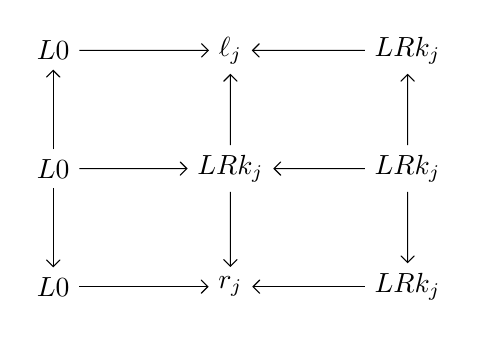
\begin{tikzpicture}[scale=0.75]
  \begin{scope}
    \node (1t) at (0,4) {$ L0 $};
    \node (2t) at (3,4) {$ \ell_j $};
    \node (3t) at (6,4) {$ LRk_j $};
    \node (1m) at (0,2) {$ L 0 $};
    \node (2m) at (3,2) {$ LRk_j $};
    \node (3m) at (6,2) {$ LRk_j $};
    \node (1b) at (0,0) {$ L0 $};
    \node (2b) at (3,0) {$ r_j $};
    \node (3b) at (6,0) {$ LRk_j $};
    \draw [cd] (1t) edge (2t);
    \draw [cd] (3t) edge (2t);
    \draw [cd] (1m) edge (2m);
    \draw [cd] (3m) edge (2m);
    \draw [cd] (1b) edge (2b);
    \draw [cd] (3b) edge (2b);
    \draw [cd] (1m) edge (1t);
    \draw [cd] (1m) edge (1b);
    \draw [cd] (2m) edge (2t);
    \draw [cd] (2m) edge (2b);
    \draw [cd] (3m) edge (3t);
    \draw [cd] (3m) edge (3b);
  \end{scope}
\end{tikzpicture}\end{center}

Then, $ g \rightsquigarrow^\ast h$ if and only
if there is a square
%
  \begin{center} 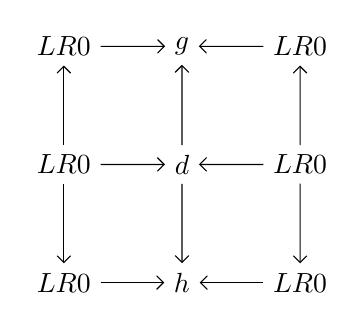
\begin{tikzpicture}[scale=0.75]
    \node (1t) at (0,4) {$ LR 0 $};
    \node (2t) at (2,4) {$ g $};
    \node (3t) at (4,4) {$ LR 0 $};
    \node (1m) at (0,2) {$ LR 0 $};
    \node (2m) at (2,2) {$ d $};
    \node (3m) at (4,2) {$ LR 0 $};
    \node (1b) at (0,0) {$ LR 0 $};
    \node (2b) at (2,0) {$ h $};
    \node (3b) at (4,0) {$ LR 0 $};
    % 
    \draw [cd] (1t) to node [] {\scriptsize{$  $}} (2t);
    \draw [cd] (3t) to node [] {\scriptsize{$  $}} (2t);
    \draw [cd] (1m) to node [] {\scriptsize{$  $}} (2m);
    \draw [cd] (3m) to node [] {\scriptsize{$  $}} (2m);
    \draw [cd] (1b) to node [] {\scriptsize{$  $}} (2b);
    \draw [cd] (3b) to node [] {\scriptsize{$  $}} (2b);
    \draw [cd] (1m) to node [] {\scriptsize{$  $}} (1t);
    \draw [cd] (1m) to node [] {\scriptsize{$  $}} (1b);
    \draw [cd] (2m) to node [] {\scriptsize{$  $}} (2t);
    \draw [cd] (2m) to node [] {\scriptsize{$  $}} (2b);
    \draw [cd] (3m) to node [] {\scriptsize{$  $}} (3t);
    \draw [cd] (3m) to node [] {\scriptsize{$  $}} (3b);
  \end{tikzpicture} \end{center}
  % in our double
category (Theorem \ref{thm:inductive-rewriting}).
Because we have completely characterized the
language with these squares, the generating
squares provide the inductive definition. 

% ======================================
\subsection{Outline and contributions}
\label{sec:outl-contr}
% ======================================

In Section \ref{sec:RewriteTopoi}, we review
double pushout rewriting in topoi. This section
culminates in a functorial construction of the
rewrite relation.  The author is currently unaware
of any such construction in the literature.

In Section \ref{sec:StructureOfStrCsp}, we
introduce a modified definition of structured
cospans. They are placed as arrows into the
category $ _L\Csp $ (as done by Baez and Courser)
and we introduce a new category $ _L\StrCsp $ in
which they are objects. The main result of this
section is that $ _L\StrCsp $ is a topos (Theorem
\ref{thm:strcsp-istopos}) that is
constructed functorially in $ L $ (Theorem
\ref{thm:strcsp-isfunctorial}).

The theory of double pushout rewriting is
introduced to structured cospans in Section
\ref{sec:RewritingStrCsp}. This does not entail
simply restricting the theory of rewriting in a
topos to structured cospans, but requires that we
accommodate the added compositional
structure. The layout of this section echos the
review of DPO rewriting in Section
\ref{sec:RewriteTopoi}. We give a functorial
construction of the language for a structured
cospan grammar using double categories (Theorems
\ref{thm:StrCsp_Lang_functorial} and
\ref{thm:StrCspLang_Encodes_RewrRel}).

In their foundational paper on graph rewriting,
Ehrig, Pfender, and Schneider classify the expressiveness of
several types of grammars
\parencite[Prop.~3.3]{Ehrig_GraphGram}. We generalize
this result to certain grammars on topoi in
Section \ref{sec:gen-result-graph-rewriting}
(Theorem
\ref{thm:production-same-rewrite-relation-as-discrete}).

Finally, in Section \ref{sec:charRewrRelat}, we
use rewriting structured cospans to provide an
inductive viewpoint of rewriting in topoi (Theorem
\ref{thm:inductive-rewriting}). 

% =======================================
\subsection{On exposition}
\label{sec:word-about-expos}
% =======================================

In this paper, we move through three levels of
abstraction. The most abstract involves working
in a topos.  The intermediate level
involves working with the notion of a system
that can connect together with other compatible
systems. By a system, we mean a collection of
entities that are somehow related. Examples
include social systems, electrical systems,
physical systems, etc.  At our least
abstract, we work with a particular system, such
as the internet, which serves as a running example
throughout.

The reason we speak in terms of systems is to
make clear the motivation for structured cospans:
adding compositionality to network theory.  We
jump between these three levels of abstraction in
a casual, but deliberate, manner. 

% =======================================
\subsection{Acknowledgments}
\label{sec:acknowledgements}
% =======================================

The author would like to thank John Baez for the many
helpful conversations during the preparation of this paper.


%% ===================================
%% Rewriting in Topoi
%% ===================================
\section{Rewriting in topoi}
\label{sec:RewriteTopoi}

A common tool to model a system of objects that
are somehow related is the graph. A
graphical model offers a rich theory to any
system's analysis. One fruit of this theory,
called double pushout (DPO) graph rewriting,
provides an algebraic method to determine whether
two systems are semantically equivalent. An
example from electrical engineering is the
equivalence between two resistors $ R_1 $ and $ R_2 $ wired in series
and a single resistor $ R_1 + R_2 $.

Double pushout rewriting has an established
literature, so we use the current section to cover
the fundamentals and to establish our conventions.
The interested reader can see Ehrig, et.\ al.\
\parencite{Ehrig_GraphGram} to learn about graph
rewriting or Lack and Soboci\'{n}ski
\parencite{LackSobo_Adhesive} for an axiomatic approach
based on \emph{adhesive categories}. Here, instead
of working with the full generality offered by
adhesiveness, we work inside of a
topos. This allows us to reap the benefits from a
rich rewriting theory because topoi are
adhesive \parencite{LackSobo_TopsIsAdh}, while
retaining the technical requirements for our
constructions to work. Henceforth, every category
is a topos.

Rewriting starts with the notion of a \df{rewrite rule}, or
simply \df{rule}. This is a span $\ell \gets k \to r$
with two monic arrows. The interpretation of this rule is that
$ \ell $ can be replaced by $ r $ and $ k $ is the part of
$ \ell $ that does not change.

For example, suppose we wanted to enumerate paths
via links between two pages of a website. One way
to do this is to model the internet as a graph
where nodes correspond to websites and edges to
links.  In particular, our graph should have no
self-loops. Otherwise, two nodes would either be
connected by no paths or by infinitely many paths,
thus rendering counting useless.  To remove loops,
we can introduce the rule
\begin{equation}\label{eq:squashLoopRule}
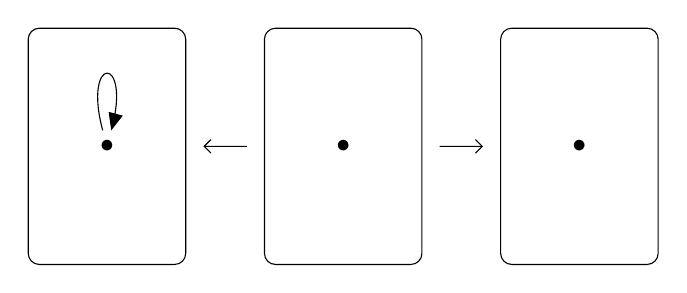
\begin{tikzpicture}
    \draw [rounded corners]
      (-1,-1) rectangle (1,2);
    \node (a)  at (0,0.5)   {$ \bullet $};
    \node (lr) at (1.1,0.5) {};  
    \draw [graph,loop above] (a) to (a);
    %
    \draw [rounded corners]
      (2,-1) rectangle (4,2);
    \node (b)  at (3,0.5)   {$ \bullet $};
    \node (ml) at (1.9,0.5) {};
    \node (mr) at (4.1,0.5) {};
    %
    \draw [rounded corners]
      (5,-1) rectangle (7,2);
    \node (c)  at (6,0.5) {$ \bullet $};
    \node (rl) at (4.9,0.5) {};
    %
    \draw [cd]
      (ml) edge node[]{$  $} (lr)
      (mr) edge node[]{$  $} (rl); 
 \end{tikzpicture}
 \end{equation}   

Typically, a collection of rewrite rules is packaged
together with a given system. Resistor circuits have
parallel, series, and star rules. Word processors replace
misspelled words with their correction. Calculators replace
the string $\type{2+2}$ with the string $ \type{4} $. We
formalize this idea with the following definition.

\begin{definition}[Grammar] \label{def:grammar} A
  \df{grammar} is a topos $ \T $ together with a
  finite set of rules
  $ P \bydef \{ \spn{\ell_j}{k_j}{r_j} \} $. A
  morphism of grammars
  $ ( \cat{S} , P ) \to ( \T , Q ) $ is a pullback
  and pushout preserving functor
  $ F \from \cat{S} \to \T $ such that $ Q $
  contains the image of $ P $. These form a
  category $ \Gram $.
\end{definition}

Returning to our model of the internet, we might consider the
grammar $ ( \Graph, P ) $ where $ P $ contains a single
rule: Rule \eqref{eq:squashLoopRule}. We can apply this rule
to suitable objects of $ \Graph $.  For instance, given a
graph $g$ with a self-loop, we can apply our rule to $ g $
and produce a new graph: $ g $ with the loop removed.

What, precisely, do we mean by ``apply''?
In general, we can \emph{apply} a rule
$ \ell \gets k \to r $ to an object $ \ell' $
using any arrow $ m \from \ell \to \ell' $ for
which there exists a pushout complement, that is
an object $ k' $ fitting into a pushout diagram
\[
  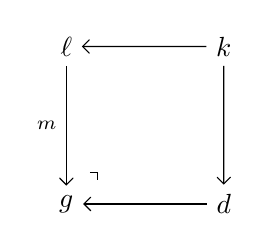
\begin{tikzpicture}
    \node (l) at (0,2) {$ \ell $};
    \node (k) at (2,2) {$ k $};
    \node (g) at (0,0) {$ g $};
    \node (d) at (2,0) {$ d $};
    \draw [cd]
       (k) edge node[]{$  $}      (l)
       (k) edge node[]{$  $}      (d)
       (l) edge node[left]{$ m $} (g)
       (d) edge node[]{$  $}      (g); 
    \draw (0.3,0.4) -- (0.4,0.4) -- (0.4,0.3);
  \end{tikzpicture}
\] A pushout
complement need not exist, but if it does and the
map $ k \to \ell $ is monic, then it is unique up to isomorphism
\parencite[Lem.~15]{LackSobo_Adhesive}.

Every application of a rule begets a new rule. Applying
$ \ell \gets k \to r $ to $\ell'$ along
$ m \from \ell \to \ell' $ induces a \df{derived rule}
$ \ell' \gets k' \to r' $ obtained as the bottom row of the
double pushout diagram \[
  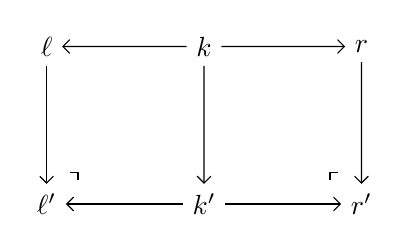
\begin{tikzpicture}
    \node (1) at (0,2) {$ \ell $};
    \node (2) at (2,2) {$ k $};
    \node (3) at (4,2) {$ r $};
    \node (4) at (0,0) {$ \ell' $};
    \node (5) at (2,0) {$ k' $};
    \node (6) at (4,0) {$ r' $};
    \draw [cd]
    (2) edge (1)
    (2) edge (3)
    (5) edge (4)
    (5) edge (6)
    (1) edge (4)
    (2) edge (5)
    (3) edge (6); 
    \draw (0.3,0.4) -- (0.4,0.4) -- (0.4,0.3);
    \draw (3.7,0.4) -- (3.6,0.4) -- (3.6,0.3);
  \end{tikzpicture}
\] This diagram expresses a three-stage process whereby
$ m $ selects a copy of $ \ell $ inside $ \ell' $, this copy
is replaced by $ r $, and the resulting object $ r' $ is
returned.  Because pushouts preserve monics in a topos, a
derived rule is, in fact, a rule.

Let us illustrate this using our graphical model
of the internet.  Rule \eqref{eq:squashLoopRule}
is applicable to any node with a loop, such as in
the double pushout diagram
\begin{equation} \label{eq:example-dpo-diagram}
 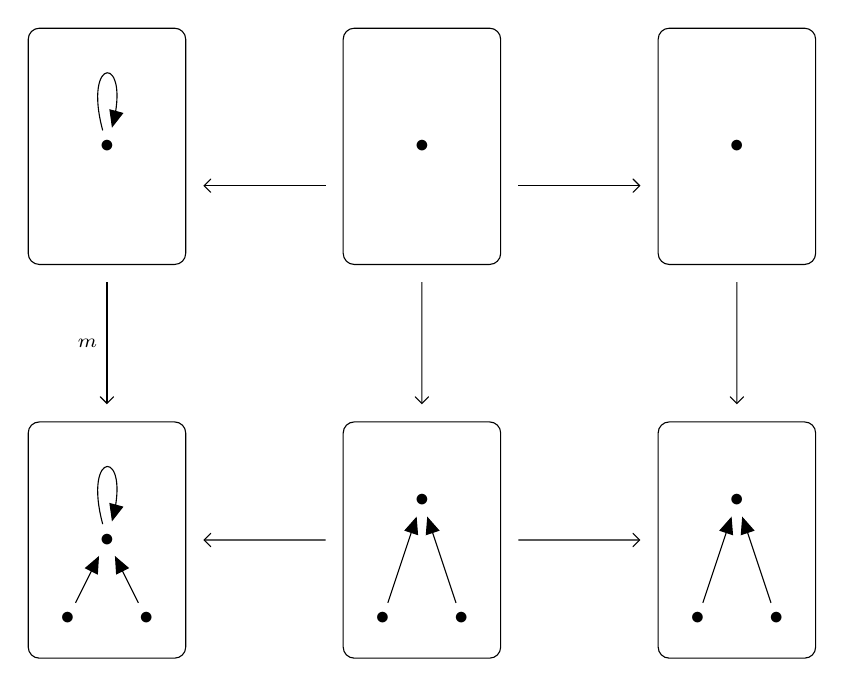
\begin{tikzpicture}
    \begin{scope} 
      \node (c) at (0,0.5) {$ \bullet $};
      \draw [graph,loop above]
        (c) edge (c);
      \draw [rounded corners]
        (-1,-1) rectangle (1,2);
      \node (01r) at (1.1,0)  {};
      \node (01b) at (0,-1.1) {};  
    \end{scope}
    %
    \begin{scope}[shift={(4,0)}]
      \node (c) at (0,0.5) {$ \bullet $};
      \draw [rounded corners]
        (-1,-1) rectangle (1,2);
      \node (11l) at (-1.1,0) {};
      \node (11r) at (1.1,0)  {};
      \node (11b) at (0,-1.1) {};
    \end{scope}
    %
    \begin{scope}[shift={(8,0)}]
      \node (c) at (0,0.5) {$ \bullet $};
      %
      \draw [rounded corners]
        (-1,-1) rectangle (1,2);
      \node (21l) at (-1.1,0) {};
      \node (21b) at (0,-1.1) {};
    \end{scope}
    %
    \begin{scope}[shift={(0,-5)}]
      \node (a) at (-0.5,-0.5) {$ \bullet $};
      \node (b) at (0.5,-0.5)  {$ \bullet $};
      \node (c) at (0,0.5)     {$ \bullet $};
      \draw [graph]
      (a) edge              (c)
      (b) edge              (c)
      (c) edge [loop above] (c);
      %
      \draw [rounded corners]
        (-1,-1) rectangle (1,2);
      \node (00t) at (0,2.1)   {};
      \node (00r) at (1.1,0.5) {};  
    \end{scope}
    %
    \begin{scope}[shift={(4,-5)}]
      \node (a) at (-0.5,-0.5) {$ \bullet $};
      \node (b) at (0.5,-0.5) {$ \bullet $};
      \node (c) at (0,1) {$ \bullet $};
      \draw [graph]
        (a) edge (c)
        (b) edge (c);
      %
      \draw [rounded corners]
        (-1,-1) rectangle (1,2);
      \node (10t) at (0,2.1)    {};
      \node (10r) at (1.1,0.5)  {};
      \node (10l) at (-1.1,0.5) {};
    \end{scope}
    %
    \begin{scope}[shift={(8,-5)}]
      \node (a) at (-0.5,-0.5) {$ \bullet $};
      \node (b) at (0.5,-0.5)  {$ \bullet $};
      \node (c) at (0,1)    {$ \bullet $};
      \draw [graph]
      (a) edge              (c)
      (b) edge              (c);
      %
      \draw [rounded corners]
        (-1,-1) rectangle (1,2);
      \node (20t) at (0,2.1)    {};
      \node (20l) at (-1.1,0.5) {};
      \end{scope}
      % 
      \draw [cd]
      (01b) edge node[left]{$ m $} (00t)
      (11b) edge (10t)
      (21b) edge (20t)
      (11l) edge (01r)
      (11r) edge (21l)
      (10l) edge (00r)
      (10r) edge (20l);
    \end{tikzpicture}
  \end{equation}

  

In the bottom left graph, we have modeled a
portion of the internet where one webpage has a
link to itself.  By applying Rule
\eqref{eq:squashLoopRule} to this graph, we obtain
a model of this same portion of the internet minus
this link. If we were counting paths between
webpages, the new model is preferable.  

A grammar $( \T,P )$ induces a collection $dP$ of
all derived rules obtained by applying a rule in
$P$ to an object in $\T$.  We can use $dP$ to
analyze the grammar $(\T,P)$ by constructing the
`rewrite relation' $\deriv{}{}$. The meaning
of $\deriv{x}{y}$ is that we can rewrite $x$ into
$y$ by applying a sequence of rules in $dP$. To
precisely define the rewrite relation, we start by
constructing a relation $ \dderiv{}{} $ on the
objects of $ \T $ by setting
$ \dderiv{\ell'}{r'} $ if there exists a rule
$ \spn{\ell'}{k'}{r'} $ in $ dP $. For instance,
Diagram \eqref{eq:example-dpo-diagram} implies
that \[
  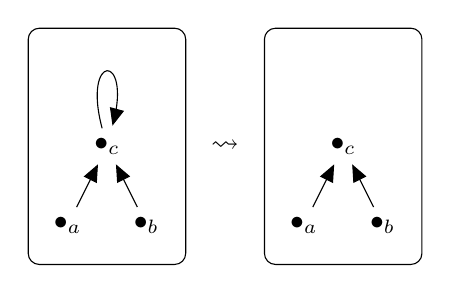
\begin{tikzpicture}
    \begin{scope}[shift={(0,0)}]
      \node (a) at (-0.5,-0.5) {$ \bullet_a $};
      \node (b) at (0.5,-0.5)  {$ \bullet_b $};
      \node (c) at (0,0.5)     {$ \bullet_c $};
      \draw [graph]
        (a) edge              (c)
        (b) edge              (c)
        (c) edge [loop above] (c); 
      %
      \draw [rounded corners]
        (-1,-1) rectangle (1,2);
    \end{scope}
    %
    \node at (1.5,0.5) {$ \dderiv{}{} $};
    %
    \begin{scope}[shift={(3,0)}]
      \node (a) at (-0.5,-0.5) {$ \bullet_a $};
      \node (b) at (0.5,-0.5)  {$ \bullet_b $};
      \node (c) at (0,0.5)       {$ \bullet_c $};
      \draw [graph]
        (a) edge              (c) 
        (b) edge              (c);
      \draw [rounded corners]
        (-1,-1) rectangle (1,2);
    \end{scope}
  \end{tikzpicture}
\] However,
$ \dderiv{}{} $ does not capture enough
information about $( \T,P )$, which is why we
define the \df{rewrite relation} $ \deriv{}{} $ to
be the reflexive and transitive closure of
$ \dderiv{}{} $.

The rewrite relation can be encoded as arrows in a
category via a functorial construction we call the
``language functor''. In the rewriting literature,
the terms ``language'' and ``rewrite relation''
are interchangeable. However, we give them slightly
different meanings in order to help orient the
reader. Namely, we use ``rewrite relation'' when
giving a relational perspective and ``language''
when giving the category theoretical perspective.

\begin{theorem}
  \label{thm:Lang_from_Gram_to_Cat}
  Let $ (\T,P) $ be a grammar and $ dP $ be the
  set of all rules derived from $ ( \T,P )
  $. Define a relation $ \dderiv{}{} $ on objects
  of $ \T $ by $ \dderiv{\ell'}{r'} $ if and only
  if there is a rule $ \ell' \gets k' \to r' $ in
  $ dP $.

  There exists a category $ \Lang (\T,P) $
  whose objects are those of $ \T $ and arrows are
  generated by the relation $ \dderiv{x}{y}
  $. Given a morphism of grammars
  $ F \from (\T,P) \to (\T',P') $, there is a
  functor
  $ \Lang (F) \from \Lang (\T,P) \to \Lang
  (\T',P') $ defined on objects by
  $ x \mapsto Fx $ and on arrows by extending from
  $ (\dderiv{x}{y}) \mapsto ( \dderiv{Fx}{Fy} )
  $. This defines a functor
  $ \Lang \from \Gram \to \Cat $
\end{theorem}

\begin{corollary}
  Let $ \deriv{}{} $ be the rewrite relation for
  $ ( \T,P ) $ and let $ x $ and $ y $ be objects
  of $ \T $. There is an arrow $ x \to y $ in
  $ \Lang (\T,P) $ if and only if
  $ \deriv{x}{y} $.
\end{corollary}

\begin{proof}
  Sufficiency follows by construction. For
  necessity, suppose $\deriv{x}{y}$. Then either
  $x=y$ and the identity arrow in $\Lang(\T,P)$ is
  the arrow we seek, or there is a sequence
  $x \rightsquigarrow x_1 \rightsquigarrow \dotsm
  \rightsquigarrow x_n \rightsquigarrow y $ which
  gives the sequence of arrows
  $x \to x_1 \to \dotsm \to x_n \to y$ in
  $\Lang (\T,P)$ whose composite is the arrow we
  seek.
\end{proof}

Though there is more to the theory of rewriting
that providing in this section, we have developed
enough of the theory to continue our goal of
introducing rewriting to structured cospans.

%% ===========================================
\section{Structured cospans form a topos}
\label{sec:StructureOfStrCsp}
%% ===========================================

Every topos supports a rich rewriting theory. This
fact underpins our efforts to introduce rewriting
to structured cospans. And so, in this section, we
reintroduce the notion of structured cospans and
find sufficient conditions for them to form a topos.

Baez and Courser \parencite{bc_strCsp} introduced
structured cospans as a framework to study open
systems.  A system is \df{open} when
equipped with a mechanism by which it can connect
to any compatible system.  For example, a vacuum cleaner can
connect with the electrical grid via an electrical
socket. A pulley system can connect to a
mechanical motor. An open system stands in
contrast to a closed system that cannot
interact with its outside environment.

In order to rewrite structured cospans in the
sense of Section {\ref{sec:RewriteTopoi}}, they
must form a topos.  To achieve this, we impose
stronger conditions than given by Baez and
Courser.  To specify these conditions, we use what
is known as a geometric morphism. This is an adjunction
$$\adjunction{\X}{L}{R}{\A}$$ between topoi with $
L $ left exact. 

%% define structured cospans
\begin{definition}
  Fix a geometric morphism
  $ L \dashv R \from \X \to \A $. An
  \df{$ L $-structured cospan}, or simply
  \df{structured cospan}, is a diagram  $ La \to x
  \gets Lb $ in $ \X $. 
\end{definition}

To interpret $ \spn{La}{x}{Lb} $ as an open system, take $x$
to represent the system with inputs $ La $ chosen by the
arrow $ La \gets x$ and outputs $ Lb $ chosen by $ Lb \to x $.
This open system can now connect to any other open system
with inputs $ Lb $, say $ \spn{Lb}{y}{Lc} $. We form the
\emph{composite} of the two open systems by connecting $ x $
to $ y $ along their common interface $ Lb $.
Mathematically, this amounts to taking the pushout of $ x $
and $ y $ over $ Lb $, thus giving the composite system
$ \spn{La}{x+_{Lb}y}{Lc} $.

We intentionally chose the term ``composite system'' to
suggest that structured cospans are the arrows of some
category.  Indeed, this is the case.

%% define category w str cospans as arrows
\begin{definition} \label{def:LCsp_category} Fix a geometric
  morphism $ L \dashv R \from \X \to \A $.  Denote by
  $ _L \Csp $ the category whose objects are those of $ \A $
  and whose arrows from $ a $ to $ b $ are (isomorphism
  classes of) structured cospans $ La \to x \gets Lb $.
\end{definition}

For $ _L \Csp $ to form a category, we do not
require the full strength of the conditions listed in
Definition \ref{def:LCsp_category}---Baez and
Courser do not ask this much---but remember, we
are aiming to form a topos of structured cospans.

\begin{example} \label{ex:open_graphs}

  Structured cospans can be used to define open
  graphs.  A graph is open when equipped with two
  subsets of nodes, one set serving as inputs and
  the other as outputs. When the inputs of one
  open graph coincide with the outputs of another,
  they can be composed. For example, the pair of
  open graphs \begin{center}
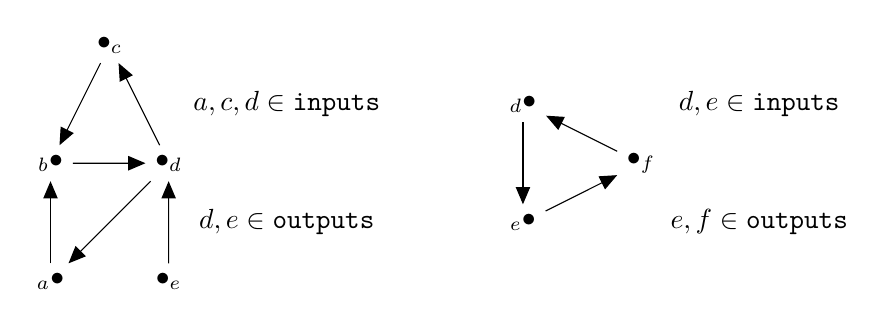
\begin{tikzpicture}[scale=0.75]
  \begin{scope}
    \node (1) at (0,0) {{$ _a \bullet $}};
    \node (2) at (0,2) {{$ _b \bullet $}};
    \node (3) at (2,2) {{$ \bullet_d $}};
    \node (4) at (2,0) {{$ \bullet_e $}};
    \node (5) at (1,4) {{$ \bullet_c $}};
    %
    \draw [graph]
    (1) edge[] (2)
    (2) edge[] (3)
    (3) edge[] (1)
    (4) edge[] (3)
    (3) edge[] (5)
    (5) edge[] (2);
    %
    \node () at (4,3) {$ a,c,d \in \mathtt{ inputs} $ };
    \node () at (4,1) {$ d,e \in \mathtt{ outputs} $};
  \end{scope}
  % 
  \begin{scope}[shift={(8,0)}]
    \node (1) at (0,3) {{$ _{d} \bullet $}};
    \node (2) at (0,1) {{$ _{e} \bullet $}};
    \node (3) at (2,2) {{$ \bullet_{f} $}};
    %
    \draw [graph] 
    (1) edge[] (2)
    (2) edge[] (3)
    (3) edge[] (1); 
    %
    \node () at (4,3) {$ d,e \in \mathtt{ inputs} $};
    \node () at (4,1) {$ e,f \in \mathtt{ outputs} $};  
  \end{scope}
\end{tikzpicture}
\end{center}  
  compose by glueing the corresponding nodes
  together, forming the new open graph
  \begin{center}
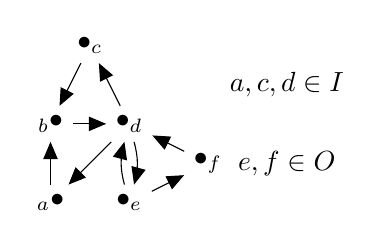
\begin{tikzpicture}[scale=0.5]
  \node (1) at (0,0) {{$ _a \bullet $}};
  \node (2) at (0,2) {{$ _b \bullet $}};
  \node (3) at (2,2) {{$ \bullet_{d} $}};
  \node (4) at (2,0) {{$ \bullet_{e} $}};
  \node (5) at (1,4) {{$ \bullet_c $}};
  \node (6) at (4,1) {{$ \bullet_f$}};
  % 
  \draw [graph]
    (1) edge[] (2)
    (2) edge[] (3)
    (3) edge[] (1)
    (3) edge[bend left=15] (4)
    (3) edge[] (5)
    (5) edge[] (2)
    (4) edge[bend left=15] (3)
    (4) edge[] (6)
    (6) edge[] (3); 
  % 
  \node () at (6,3) {$ a,c,d \in I $};
  \node () at (6,1) {$ e,f \in O $};
\end{tikzpicture}  
\end{center} To define an open
  graph as a structured cospan, consider the
  geometric
  morphism $$\adjunction{\Graph}{L}{R}{\Set}$$
  where $ L $ is the discrete graph functor and
  $ R $ forgets the graph edges. The above open
  graphs can be presented as the structured
  cospans \[
  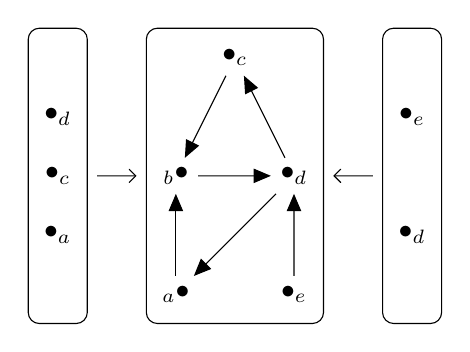
\begin{tikzpicture}[
    baseline=(current bounding box.center),
    scale=0.75]
  \begin{scope}
    \node () at (0,1) {$ \bullet_a $};
    \node () at (0,2) {$ \bullet_c $};
    \node () at (0,3) {$ \bullet_d $};
    \draw [rounded corners]
    (-0.5,-0.5) rectangle (0.5,4.5);
    \node (InDom) at (0.5,2) {};
  \end{scope}
  \begin{scope}[shift={(2,0)}]
    \node (1) at (0,0) {{$ _a \bullet $}};
    \node (2) at (0,2) {{$ _b \bullet $}};
    \node (3) at (2,2) {{$ \bullet_d $}};
    \node (4) at (2,0) {{$ \bullet_e $}};
    \node (5) at (1,4) {{$ \bullet_c $}};
    %
    \draw [graph]
    (1) edge[] (2)
    (2) edge[] (3)
    (3) edge[] (1)
    (4) edge[] (3)
    (3) edge[] (5)
    (5) edge[] (2);
    %
    \draw [rounded corners]
    (-0.5,-0.5) rectangle (2.5,4.5);
    \node (InCod) at (-0.5,2) {};
    \node (OutCod) at (2.5,2) {};
  \end{scope}
  \begin{scope}[shift={(6,0)}]
    \node () at (0,1) {$ \bullet_d $};
    \node () at (0,3) {$ \bullet_e $};
    \draw [rounded corners]
    (-0.5,-0.5) rectangle (0.5,4.5);
    \node (OutDom) at (-0.5,2) {};
  \end{scope}
  \draw [cd]
  (InDom) edge[] (InCod)
  (OutDom) edge[] (OutCod);
\end{tikzpicture}
%
\quad \text{ and } \quad
%
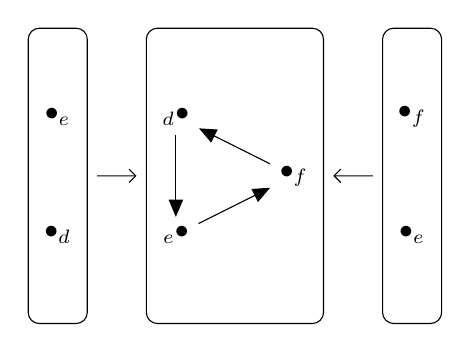
\begin{tikzpicture}[
  baseline=(current bounding box.center),
  scale=0.75]
  \begin{scope}
    \node () at (0,1) {$ \bullet_d $};
    \node () at (0,3) {$ \bullet_e $};
    \draw [rounded corners]
    (-0.5,-0.5) rectangle (0.5,4.5);
    \node (InDom) at (0.5,2) {};
  \end{scope}
  \begin{scope}[shift={(2,0)}]
    \node (1) at (0,3) {{$ _{d} \bullet $}};
    \node (2) at (0,1) {{$ _{e} \bullet $}};
    \node (3) at (2,2) {{$ \bullet_{f} $}};
    %
    \draw [graph] 
    (1) edge[] (2)
    (2) edge[] (3)
    (3) edge[] (1); 
    %
    \draw [rounded corners]
    (-0.5,-0.5) rectangle (2.5,4.5);
    \node (InCod) at (-0.5,2) {};
    \node (OutCod) at (2.5,2) {};
  \end{scope}
  \begin{scope}[shift={(6,0)}]
    \node () at (0,1) {$ \bullet_e $};
    \node () at (0,3) {$ \bullet_f $};
    \draw [rounded corners]
    (-0.5,-0.5) rectangle (0.5,4.5);
    \node (OutDom) at (-0.5,2) {};
  \end{scope}
  \draw [cd]
  (InDom) edge[] (InCod)
  (OutDom) edge[] (OutCod);
\end{tikzpicture}
\]
 with
  composite \[
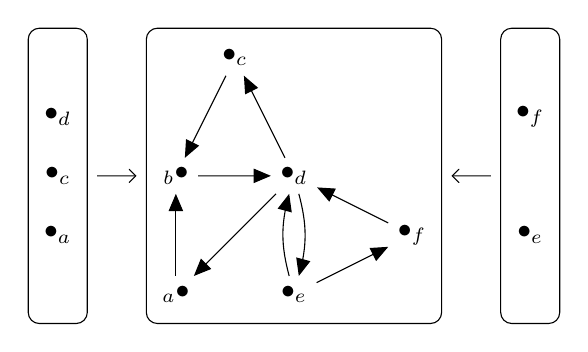
\begin{tikzpicture}[scale=0.75]
  \begin{scope}
    \node () at (0,1) {$ \bullet_a $};
    \node () at (0,2) {$ \bullet_c $};
    \node () at (0,3) {$ \bullet_d $};
    \draw [rounded corners]
    (-0.5,-0.5) rectangle (0.5,4.5);
    \node (InDom) at (0.5,2) {};
  \end{scope}
  \begin{scope}[shift={(2,0)}]
  \node (1) at (0,0) {{$ _a \bullet $}};
  \node (2) at (0,2) {{$ _b \bullet $}};
  \node (3) at (2,2) {{$ \bullet_{d} $}};
  \node (4) at (2,0) {{$ \bullet_{e} $}};
  \node (5) at (1,4) {{$ \bullet_c $}};
  \node (6) at (4,1) {{$ \bullet_f$}};
  % 
  \draw [graph]
    (1) edge[] (2)
    (2) edge[] (3)
    (3) edge[] (1)
    (3) edge[bend left=15] (4)
    (3) edge[] (5)
    (5) edge[] (2)
    (4) edge[bend left=15] (3)
    (4) edge[] (6)
    (6) edge[] (3);  
    %
    \draw [rounded corners]
    (-0.5,-0.5) rectangle (4.5,4.5);
    \node (InCod) at (-0.5,2) {};
    \node (OutCod) at (4.5,2) {};
  \end{scope}
  \begin{scope}[shift={(8,0)}]
    \node () at (0,1) {$ \bullet_e $};
    \node () at (0,3) {$ \bullet_f $};
    \draw [rounded corners]
    (-0.5,-0.5) rectangle (0.5,4.5);
    \node (OutDom) at (-0.5,2) {};
  \end{scope}
  \draw [cd]
  (InDom) edge[] (InCod)
  (OutDom) edge[] (OutCod);
\end{tikzpicture}
\] In this
  example, the category $ _L\Csp $ has sets for
  objects and open graphs for arrows.
\end{example}

Recall that, in Section \ref{sec:RewriteTopoi}, we saw
that rewriting operates on the objects of a topos,
not the arrows. Therefore, we cannot hope to rewrite
structured cospans inside the category $ _L\Csp $. Our
task, now, is to define a category where structured
cospans are objects. Then we can show that category to be a
topos.

% define L-structured cospan morphism
\begin{definition} \label{df:morph-of-strcsp} Let
  $ L \dashv R \from \X \to \A $ be geometric
  morphism. Define $ _L \StrCsp $ to be the category whose
  objects are $ L $-structured cospans and arrows from
  $ La \to x \gets Lb $ to $ Lc \to y \gets Ld $ are triples
  of arrows $ ( f,g,h ) $ fitting into the commuting diagram
  \[
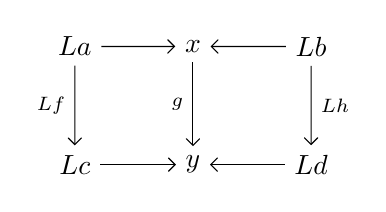
\begin{tikzpicture}[scale=0.75]
  \node (1) at (-2,2) {\( La \)};
  \node (2) at (0,2) {\( x \)};
  \node (3) at (2,2) {\( Lb \)};
  \node (4) at (-2,0) {\( Lc \)};
  \node (5) at (0,0) {\( y \)};
  \node (6) at (2,0) {\( Ld \)};
  \draw [cd]
    (1) edge node[]{} (2)
    (3) edge node[]{} (2)
    (4) edge node[]{} (5)
    (6) edge node[]{} (5)
    (1) edge node[left]{$Lf$}  (4)
    (2) edge node[left]{$g$}   (5)
    (3) edge node[right]{$Lh$} (6);
\end{tikzpicture}
\]
\end{definition}

%% structured cospans form a topos
\begin{theorem} \label{thm:strcsp-istopos} Let
  $ L \dashv R \from \X \to \A $ be a geometric
  morphism.  The category $ _{L}\StrCsp $ is a
  topos.
\end{theorem}
\begin{proof}
  By adjointness, $ _{L}\StrCsp $ is equivalent to
  the category whose objects are cospans of form
  $ a \to Rx \gets b $ and morphisms are triples
  $ ( f,g,h ) $ fitting into the commuting diagram
  \begin{center}
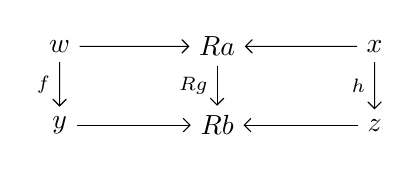
\begin{tikzpicture}
  \node (1) at (-2,1) {\( w \)};
  \node (2) at (0,1) {\( Ra \)};
  \node (3) at (2,1) {\( x \)};
  \node (4) at (-2,0) {\( y \)};
  \node (5) at (0,0) {\( Rb \)};
  \node (6) at (2,0) {\( z \)};
  \draw [cd] (1) to  node [] {} (2);
  \draw [cd] (3) to node [] {} (2);
  \draw [cd] (4) to node [] {} (5);
  \draw [cd] (6) to node [] {} (5);
  \draw [cd] (1) to node [left] {$f$} (4);
  \draw [cd] (2) to node [left] {$Rg$} (5);
  \draw [cd] (3) to node [left] {$h$} (6); 
\end{tikzpicture}
\end{center} This, in
  turn, is equivalent to the comma category
  $ ( \A \times \A \downarrow \Delta R ) $ where
  $ \Delta \from \A \to \A \times \A $ is the
  diagonal functor, a right adjoint. Because
  $ \Delta R $ is a right adjoint,
  $ ( \A \times \A \downarrow \Delta R ) $ is an
  Artin glueing \parencite{Wraith_ArtinGlue}, therefore
  a topos.
\end{proof}

Not only is $ _L\StrCsp $ a topos, but it is constructed functorially.

\begin{theorem} \label{thm:strcsp-isfunctorial}
  Denote by $ \Topos $ the category of topoi and
  geometric morphisms. There is a functor
  \[
    _{(-)}\StrCsp
      \from [\bullet \to \bullet, \Topos ]
      \to   Topos
  \]
  defined by \begin{center}
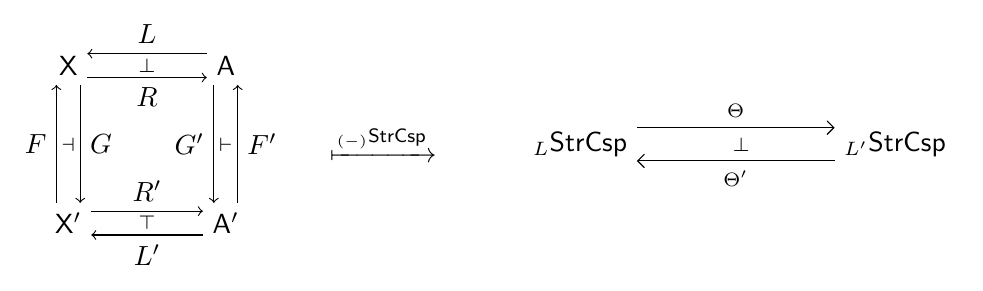
\begin{tikzpicture}
  \begin{scope}
    \node (1) at (-1,1) {$\X$};
    \node (2) at (-1,-1) {$\X'$};
    \node (3) at (1,1) {$\A$};
    \node (4) at (1,-1) {$\A'$};
    \draw [transform canvas = {xshift=1ex}, ->]
    (1) edge node [right] {$G$} (2);
    \draw [transform canvas = {xshift=-1ex}, ->]    
    (2)  edge node [left]  {$F$}  (1);
    \draw [transform canvas = {yshift=1ex}, ->]
    (3)  edge node [above] {$L$}  (1);
    \draw [transform canvas = {yshift=-1ex}, ->]   
    (1)  edge node [below] {$R$}  (3);
    \draw [transform canvas = {yshift=1ex}, ->]
    (2)   edge node [above] {$R'$} (4);
    \draw [transform canvas = {yshift=-1ex}, ->]
    (4) edge node [below] {$L'$} (2);
    \draw [transform canvas = {xshift=1ex}, ->]
    (4)   edge node [right] {$F'$} (3);
    \draw [transform canvas = {xshift=-1ex}, ->]
    (3) edge node [left]  {$G'$} (4);
    \node (5) at (0,-1) {\scriptsize{\( \top \)}};
    \node (6) at (0,1) {\scriptsize{\( \perp \)}};
    \node (7) at (-1,0) {\scriptsize{\( \dashv \)}};
    \node (8) at (1,0) {\scriptsize{\( \vdash \)}};
  \end{scope}
  % 
  \begin{scope}[shift={(3,0)}]
    \node (1) at (0,0) { $\xmapsto{ _{(-)}\StrCsp }$ };
  \end{scope}
  % 
  \begin{scope}[shift={(5.5,0)}]
    \node (1) [] at (0,0) {\( _{L}\StrCsp \)};
    \node (2) [] at (4,0) {\( _{L'}\StrCsp \)};
    \node (3) at (2,0) {\scriptsize{ \( \perp \) }};
    \draw [cd]
      ([yshift=1pt]1.east) to
      node [above] {$\Theta$}
      ([yshift= 1pt]2.west);
    \draw [cd]
    ([yshift= -1pt]2.west) to
    node [below] {$\Theta'$}
    ([yshift= -1pt]1.east);  
  \end{scope}
\end{tikzpicture}
\end{center} which is
  in turn given by \begin{center}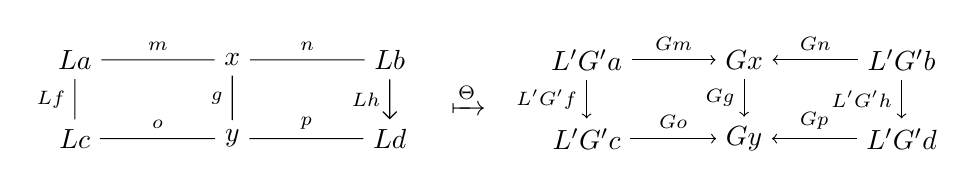
\begin{tikzpicture}
    \begin{scope}
      \node (1) at (-2,1) {\( La \)};
      \node (2) at (0,1) {\( x \)};
      \node (3) at (2,1) {\( Lb \)};
      \node (4) at (-2,0) {\( Lc \)};
      \node (5) at (0,0) {\( y \)};
      \node (6) at (2,0) {\( Ld \)};
      \draw [cd]
        (1) to node [above] {$ m $}  (2)
        (3) to node [above] {$ n $}  (2)
        (4) to node [above] {$ o $}  (5)
        (6) to node [above] {$ p $}  (5)
        (1) to node [left]  {$ Lf $} (4)
        (2) to node [left]  {$ g $}  (5)
        (3) to node [left]  {$ Lh $} (6);
    \end{scope}
    % 
    \begin{scope}[shift={(3,0)}]
      \node (1) at (0,0.5) { $ \xmapsto{ \Theta } $ };
    \end{scope}
    % 
    \begin{scope}[shift={(6.5,0)}]
        \node (1) at (-2,1) {\( L'G'a \)};
        \node (2) at (0,1) {\( Gx \)};
        \node (3) at (2,1) {\( L'G'b \)};
        \node (4) at (-2,0) {\( L'G'c \)};
        \node (5) at (0,0) {\( Gy \)};
        \node (6) at (2,0) {\( L'G'd \)};
        \draw [->] (1) to node [above] {\scriptsize{\( Gm \)}} (2);
        \draw [->] (3) to node [above] {\scriptsize{\( Gn \)}} (2);
        \draw [->] (4) to node [above] {\scriptsize{\( Go \)}} (5);
        \draw [->] (6) to node [above] {\scriptsize{\( Gp \)}} (5);
        \draw [->] (1) to node [left] {\scriptsize{\( L'G'f \)}} (4);
        \draw [->] (2) to node [left] {\scriptsize{\( Gg \)}} (5);
        \draw [->] (3) to node [left] {\scriptsize{\( L'G'h \)}} (6);  
    \end{scope}
  \end{tikzpicture}\end{center} and
  \begin{center}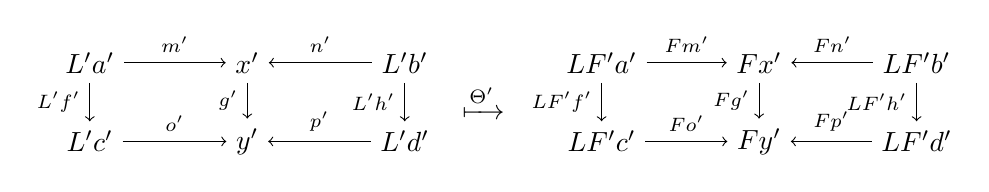
\begin{tikzpicture}
    \begin{scope}
      \node (1) at (-2,1) {\( L'a' \)};
      \node (2) at (0,1) {\( x' \)};
      \node (3) at (2,1) {\( L'b' \)};
      \node (4) at (-2,0) {\( L'c' \)};
      \node (5) at (0,0) {\( y' \)};
      \node (6) at (2,0) {\( L'd' \)};
      \draw [->] (1) to node [above] {\scriptsize{\( m' \)}} (2);
      \draw [->] (3) to node [above] {\scriptsize{\( n' \)}} (2);
      \draw [->] (4) to node [above] {\scriptsize{\( o' \)}} (5);
      \draw [->] (6) to node [above] {\scriptsize{\( p' \)}} (5);
      \draw [->] (1) to node [left] {\scriptsize{\( L'f' \)}} (4);
      \draw [->] (2) to node [left] {\scriptsize{\( g' \)}} (5);
      \draw [->] (3) to node [left] {\scriptsize{\( L'h' \)}} (6);
    \end{scope}
    %
    \begin{scope}[shift={(3,0)}]
      \node (1) at (0,0.5) { $ \xmapsto{ \Theta' } $ };
    \end{scope}
    % 
    \begin{scope}[shift={(6.5,0)}]
        \node (1) at (-2,1) {\( LF'a' \)};
        \node (2) at (0,1) {\( Fx' \)};
        \node (3) at (2,1) {\( LF'b' \)};
        \node (4) at (-2,0) {\( LF'c' \)};
        \node (5) at (0,0) {\( Fy' \)};
        \node (6) at (2,0) {\( LF'd' \)};
        \draw [->] (1) to node [above] {\scriptsize{\( Fm' \)}} (2);
        \draw [->] (3) to node [above] {\scriptsize{\( Fn' \)}} (2);
        \draw [->] (4) to node [above] {\scriptsize{\( Fo' \)}} (5);
        \draw [->] (6) to node [above] {\scriptsize{\( Fp' \)}} (5);
        \draw [->] (1) to node [left] {\scriptsize{\( LF'f' \)}} (4);
        \draw [->] (2) to node [left] {\scriptsize{\( Fg' \)}} (5);
        \draw [->] (3) to node [left] {\scriptsize{\( LF'h' \)}} (6);  
    \end{scope}
  \end{tikzpicture}\end{center}
\end{theorem}
\begin{proof}
  In light of Theorem \ref{thm:strcsp-istopos}, it suffices
  to show that $ \Theta \dashv \Theta' $ gives a geometric
  morphism.

  Let $ \ell $ denote the $ L $-structured cospans
  $ La \to x \gets Lb$ and $\ell'$ denote the
  $ L' $-structured cospan $ L'a' \to x' \gets L'b'$. Denote
  the unit and counit for $F \dashv G$ by $ \eta $,
  $ \varepsilon $ and for $ F' \dashv G' $ by $ \eta' $,
  $ \varepsilon' $.  The assignments
  \begin{align*}
    \left( (f,g,h)\from\ell\to\Theta'\ell' \right)
      & \mapsto
        \left( (\epsilon'\circ F'f,
        \epsilon\circ Fg,
        \epsilon'\circ F'h )
        \from\Theta\ell\to\ell'\right) \\
    \left( (f',g',h')\from\Theta\ell\to\ell'\right)
      & \mapsto
        \left( (G'f'\circ\eta',Gg'\circ\eta,G'h'\circ\eta')
        \from\ell\to\Theta'\ell'\right) 
  \end{align*}  
  give a bijection
  $ \hom (\Theta\ell,\ell') \simeq \hom (\ell,\Theta'\ell'
  )$. Moreover, it is natural in $\ell$ and $\ell'$. This
  rests on the natural maps $\eta$, $\epsilon$, $\eta'$, and
  $\epsilon'$. The left adjoint $\Theta'$ preserves finite
  limits because they are taken pointwise and $ L $, $ F $,
  and $ F' $ all preserve finite limits.
\end{proof}

We end this section by organizing the categories of the form
$ _L\StrCsp $ into a 2-category. 

\begin{definition} \label{df:str_csp_category}
  Let $ L \dashv R \from \X \to \A $ and
  $ L' \dashv R' \from \X' \to \A' $ be geometric
  morphisms. A \df{morphism of structured cospan categories}
  $ _L\StrCsp \to _{L'}\StrCsp $ is pair of finitely
  continuous and cocontinuous functors
  $ F \from \X \to \X' $ and $ G \from \A \to \A' $ fitting
  into the commuting diagram
  \[
  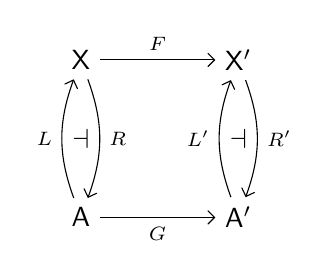
\begin{tikzpicture}
    \node (X) at (0,2) {$ \X $};
    \node (A) at (0,0) {$ \A $};
    \node (X') at (2,2) {$ \X' $};
    \node (A') at (2,0) {$ \A' $};
    \node () at (0,1) {$ \dashv $};
    \node () at (2,1) {$ \dashv $};
    \draw [cd] 
    (A) edge[bend left=20] node[left]{$ L $} (X)
    (X) edge[bend left=20] node[right]{$ R $} (A)
    (A') edge[bend left=20] node[left]{$ L' $} (X')
    (X') edge[bend left=20] node[right]{$ R' $} (A')
    (X) edge[] node[above]{$ F $} (X')
    (A) edge[] node[below]{$ G $} (A');
  \end{tikzpicture}
\]
\end{definition}

The reader may check that a morphism of structured cospan
categories gives a functor from $_L\StrCsp $ to
$ _{L'}\StrCsp $. 

Structured cospan categories fit as objects into a
2-category $ \SStrCsp $. The 1-arrows are their morphisms
and 2-arrows of type $ (F,G) \To (F',G') $ are pairs of
natural transformations $ \alpha \from F \To F' $ and
$ \beta \from G \to G'$.


%% =========================================
\section{Rewriting structured cospans}
\label{sec:RewritingStrCsp}
%% =========================================

We now know that the category $ _L\StrCsp $ of
structured cospans and their morphisms is a topos
and, therefore, support a rich rewriting
theory. In this section, we develop this theory.

\begin{definition}
  A \df{rewrite rule of structured cospans} is an
  isomorphism class of spans of structured cospans of the
  form \[
  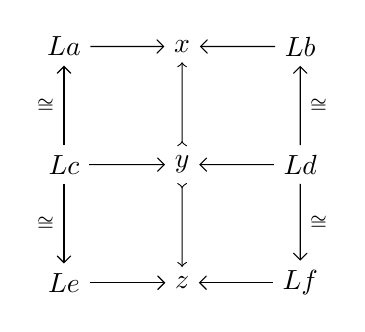
\begin{tikzpicture}[
    baseline=(current bounding box.center),
    scale=0.75]
    \node (a) at (0,4) {$ La $};
    \node (b) at (2,4) {$ x $};
    \node (c) at (4,4) {$ Lb $};
    \node (x) at (0,2) {$ Lc $};
    \node (y) at (2,2) {$ y $};
    \node (z) at (4,2) {$ Ld $};
    \node (d) at (0,0) {$ Le $};
    \node (e) at (2,0) {$ z$};
    \node (f) at (4,0) {$ Lf $};
    %    
    \draw [>->] (y) to (b);
    \draw [>->] (y) to (e);
    \draw[cd]
    (a) edge[] (b)
    (x) edge[] (y)
    (d) edge[] (e)
    (c) edge[] (b)
    (z) edge[] (y)
    (f) edge[] (e)
    (x) edge[] node[left]{$ \iso $}  (a)
    (z) edge[] node[right]{$ \iso $} (c)
    (x) edge[] node[left]{$ \iso $}  (d)
    (z) edge[] node[right]{$ \iso $} (f) ;
  \end{tikzpicture}
\]
 The marked arrows $ \rightarrowtail $ are
  monic.
\end{definition}

The conceit of this rule is that the structured
cospan in the top row of the diagram replaces the
structured cospan in the bottom row. This is
similar to a typical rewrite rule except that we
are now orienting our diagrams as
`top-replaces-bottom' instead of
`left-replaces-right'.  A non-superficial
difference is that this diagram is not merely a
span in $ _L\StrCsp $ with monic legs.  We force
the spans between the inputs and outputs to have
invertible legs, effectively preventing the
interfaces from changing in a rewrite.  This
constraint is required for the double category
$ _L\SSStrCsp $ in Definition \ref{df:L_SSStrCsp}
to satisfy the interchange law. In less technical
terms, the constraint ensures that rewriting interacts nicely
with structured cospan composition.

\begin{example}
  We illustrate this by returning to our running
  example of modeling the internet. This time,
  instead of modeling the internet with a graph,
  we use an open graph as defined via structured
  cospans in Example \ref{ex:open_graphs}. To
  remove loops in our model, we can introduce the
  rule \begin{center}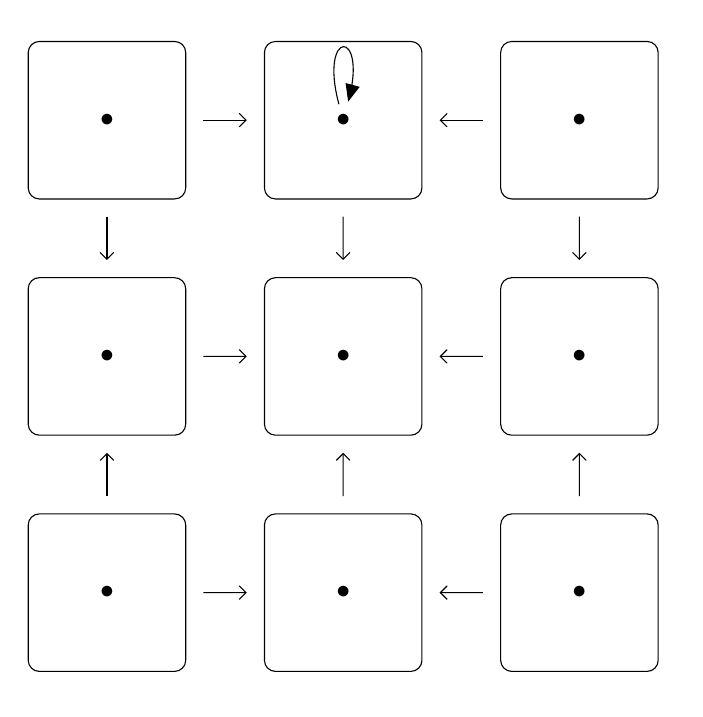
\begin{tikzpicture}
    \begin{scope}[shift={(0,0)}] % up left
      \node () at (0,0) {$ \bullet $};
      % 
      \draw [rounded corners] (-1,-1) rectangle (1,1);
      \node (00r) at (1.1,0) {};
      \node (00b) at (0,-1.1) {};  
    \end{scope}
    % 
    \begin{scope}[shift={(3,0)}] % up mid
      \node (a) at (0,0) {$ \bullet $};
      %
      \draw [graph]
        (a) edge[loop above] (a);
      %  
      \draw [rounded corners] (-1,-1) rectangle (1,1);
      \node (01l) at (-1.1,0) {};
      \node (01r) at (1.1,0)  {};
      \node (01b) at (0,-1.1) {};  
    \end{scope}
    %
    \begin{scope}[shift={(6,0)}] % up right
      \node () at (0,0) {$ \bullet $};
      %
      \draw [rounded corners] (-1,-1) rectangle (1,1);
      \node (02l) at (-1.1,0) {};
      \node (02b) at (0,-1.1) {};
    \end{scope}
    % ~~~~~~~~~~~~~~~~~~~~~~~~~~~~~
    \begin{scope}[shift={(0,-3)}] % mid left
      \node () at (0,0) {$ \bullet $};
      %
      \draw [rounded corners] (-1,-1) rectangle (1,1);
      \node (10t) at (0,1.1)   {};
      \node (10r) at (1.1,0) {};
      \node (10b) at (0,-1.1)  {};  
    \end{scope}
    %
    \begin{scope}[shift={(3,-3)}] % mid mid
      \node (a) at (0,0) {$ \bullet $};
      %
      \draw [rounded corners] (-1,-1) rectangle (1,1);
      \node (11l) at (-1.1,0) {};
      \node (11r) at (1.1,0)  {};
      \node (11t) at (0,1.1)  {};
      \node (11b) at (0,-1.1) {};  
    \end{scope}
    %
    \begin{scope}[shift={(6,-3)}] % mid right
      \node () at (0,0) {$ \bullet $};
      %
      \draw [rounded corners] (-1,-1) rectangle (1,1);
      \node (12l) at (-1.1,0) {};
      \node (12t) at (0,1.1)    {};  
      \node (12b) at (0,-1.1)   {};
    \end{scope}
    % ~~~~~~~~~~~~~~~~~~~~~
    \begin{scope}[shift={(0,-6)}] % down left
      \node () at (0,0) {$ \bullet $};
      %
      \draw [rounded corners] (-1,-1) rectangle (1,1);
      \node (20t) at (0,1.1)   {};
      \node (20r) at (1.1,0) {};
      \node (20b) at (0,-1.1)  {};  
    \end{scope}
    %
    \begin{scope}[shift={(3,-6)}] % down mid
      \node (a) at (0,0) {$ \bullet $};
      %
      \draw [rounded corners] (-1,-1) rectangle (1,1);
      \node (21l) at (-1.1,0) {};
      \node (21r) at (1.1,0)  {};
      \node (21t) at (0,1.1)  {};
      \node (21b) at (0,-1.1) {};  
    \end{scope}
    %
    \begin{scope}[shift={(6,-6)}] % down right
      \node () at (0,0) {$ \bullet $};
      %
      \draw [rounded corners]
        (-1,-1) rectangle (1,1);
      \node (22l) at (-1.1,0) {};
      \node (22r) at (1.1,0)  {};
      \node (22t) at (0,1.1)  {};
      \node (22b) at (0,-1.1) {};
    \end{scope}
    % ~~~~~~~~~~~~~~~~~~~
    \path[cd]
      (00r) edge (01l)
      (02l) edge (01r)
      (10r) edge (11l)
      (12l) edge (11r)
      (20r) edge (21l)
      (22l) edge (21r)
      (00b) edge (10t)
      (20t) edge (10b)
      (01b) edge (11t)
      (21t) edge (11b)
      (02b) edge (12t)
      (22t) edge (12b);
    \end{tikzpicture}\end{center} which
  removes a loop on any node that is both an input
  and output.
\end{example}

Before we see how to apply this rule, however, we
need to further develop our theory. Next, we look
at grammars and derived rules for structured cospans.


%% STRUCTURED COSPAN GRAMMARS ~~~~~~~~~~~~~~~~~~~~~~

\subsection{Structured cospan grammars}
\label{sec:struct-cosp-gramm}

In Definition \ref{def:grammar}, we defined a
category $ \Gram $ of grammars and their
morphisms.  Our interest now shifts to the
subcategory of $ \Gram $ spanned by the structured
cospan grammars. By a \df{structured cospan
  grammar}, we mean a structured cospan category
paired with a set of rewrite rules of structured
cospans.  A morphism a structured cospan grammars
$ (F,G) \from ( _L\StrCsp,P ) \to (_{L'}\StrCsp,
P') $ is a morphism of structured cospan
categories (Definition \ref{df:str_csp_category})
with the property that $ P' $ contains the image
of each rule in $ P $. Note that we defined a
morphism of structured cospan categories in a way
so that \[
  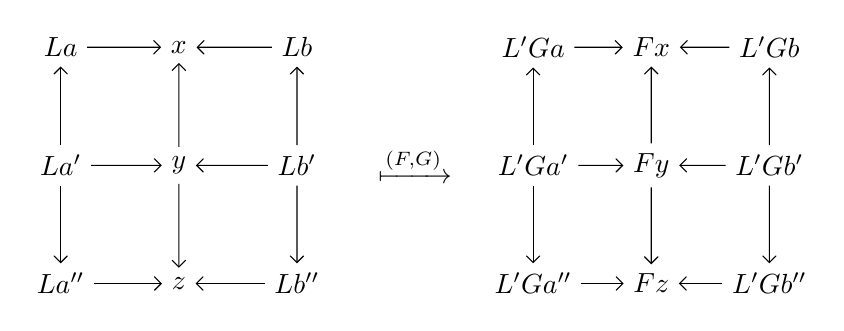
\begin{tikzpicture}[scale=0.75]    
    \begin{scope}
      \node (00) at (0,4) {$ La $};
      \node (01) at (2,4) {$ x $};
      \node (02) at (4,4) {$ Lb $};
      \node (10) at (0,2) {$ La' $};
      \node (11) at (2,2) {$ y $};
      \node (12) at (4,2) {$ Lb' $};
      \node (20) at (0,0) {$ La'' $};
      \node (21) at (2,0) {$ z $};
      \node (22) at (4,0) {$ Lb'' $};
      \path[cd]
      (00) edge[] (01)
      (02) edge[] (01)
      (10) edge[] (11)
      (12) edge[] (11)
      (20) edge[] (21)
      (22) edge[] (21)
      (10) edge[] (00)
      (11) edge[] (01)
      (12) edge[] (02)
      (10) edge[] (20)
      (11) edge[] (21)
      (12) edge[] (22);
    \end{scope}
    %
    \node () at (6,2) {$ \xmapsto{(F,G)} $};
    %
    \begin{scope}[shift={(8,0)}]
      \node (00) at (0,4) {$ L'Ga $};
      \node (01) at (2,4) {$ Fx $};
      \node (02) at (4,4) {$ L'Gb $};
      \node (10) at (0,2) {$ L'Ga' $};
      \node (11) at (2,2) {$ Fy $};
      \node (12) at (4,2) {$ L'Gb' $};
      \node (20) at (0,0) {$ L'Ga'' $};
      \node (21) at (2,0) {$ Fz $};
      \node (22) at (4,0) {$ L'Gb'' $};
      \path[cd]
      (00) edge[] (01)
      (02) edge[] (01)
      (10) edge[] (11)
      (12) edge[] (11)
      (20) edge[] (21)
      (22) edge[] (21)
      (10) edge[] (00)
      (11) edge[] (01)
      (12) edge[] (02)
      (10) edge[] (20)
      (11) edge[] (21)
      (12) edge[] (22);
    \end{scope}
\end{tikzpicture}
\]
thus ensure that the image of a rule has a form
suitable for $ P' $.

Ultimately, we want to associate a rewrite
relation to each structured cospan grammar. To do
this, we use the notion of a derived rule. But we
do need to be careful to ensure that, in the
context of structured cospans, derived rules have the
proper form.

%% DERIVED REWRITE RULES FOR STRUCTURED COSPANS ~~~~~~~

\subsection{Derived rules are rules}
\label{sec:derived-rules-are}

Derived rules emerge from pushouts, which in the
category $_L\StrCsp$ have the form
\begin{equation} \label{eq:str_csp_pushout}
  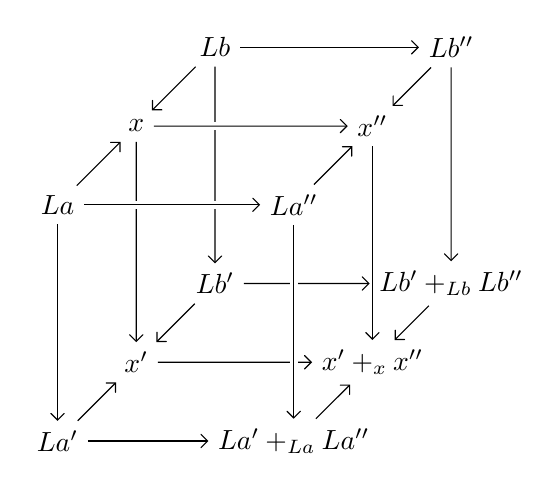
\begin{tikzpicture}[
    baseline=(current  bounding  box.center),
    scale=1]
    \node (La) at (0,3) {$ La $};
    \node (x) at (1,4) {$ x $};
    \node (Lb) at (2,5) {$ Lb $};
    %
    \node (La') at (0,0) {$ La' $};
    \node (x') at (1,1) {$ x' $};
    \node (Lb') at (2,2) {$ Lb' $};
    %
    \node (La'') at (3,3) {$ La'' $};
    \node (x'') at (4,4) {$ x'' $};
    \node (Lb'') at (5,5) {$ Lb'' $};
    % 
    \node (POa) at (3,0) {$ La'+_{La}La'' $};
    \node (POx) at (4,1) {$ x'+_xx'' $};
    \node (POb) at (5,2) {$ Lb'+_{Lb}Lb'' $};
    %
    \draw [cd]
    (La) edge[] (x)
    (Lb) edge[] (x)
    (La') edge[] (x')
    (Lb') edge[] (x') 
    (La'') edge[] (x'')
    (Lb'') edge[] (x'') 
    (POa) edge[] (POx)
    (POb) edge[] (POx)
    %
    (La) edge[] (La') 
    (La') edge[] (POa)
    %
    (x) edge[] (x')    
    (x') edge[] (POx)
    (x'') edge[] (POx)
    %
    (Lb) edge[] (Lb')
    (Lb) edge[] (Lb'')
    (Lb') edge[] (POb)
    (Lb'') edge[] (POb);
    %
    \draw [line width=1mm, white]
      (x) -- (x'')
      (La'') -- (POa)
      (La) -- (La'');
    \draw [cd]
      (x) edge[] (x'')
      (La'') edge[] (POa)
      (La) edge[] (La'');
  \end{tikzpicture}
\end{equation}
 The legs of the
span
$$\spn{La'+_{La}La''}{x'+_xx''}{Lb'+_{Lb}Lb''}$$
are induced by the universal property of the
pushouts $La'+_{La}La''$ and $Lb'+_{La}Lb''$. This
same universal property ensures that the bottom
and right faces of Diagram
\eqref{eq:str_csp_pushout} commute. Moreover, this
span is an $L$-structured cospan because as
a left adjoint $L$ preserves pushouts so is
isomorphic to
$ L(a'+_aa'') \gets x'+_xx'' \to L(b'+_bb'') $.

Consider a structured cospan rule
\begin{center}
  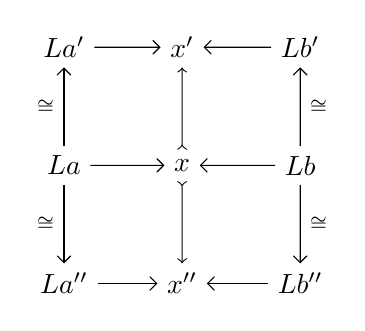
\begin{tikzpicture}[scale=0.75]
    \node (La'') at (0,0) {$ La'' $};
    \node (x'') at (2,0) {$ x'' $};
    \node (Lb'') at (4,0) {$ Lb'' $};
    \node (La) at (0,2) {$ La $};
    \node (x) at (2,2) {$ x $};
    \node (Lb) at (4,2) {$ Lb $};
    \node (La') at (0,4) {$ La' $};
    \node (x') at (2,4) {$ x' $};
    \node (Lb') at (4,4) {$ Lb' $};
    %
    \draw [cd] 
    (La) edge[] (x)
    (Lb) edge[] (x)
    (La') edge[] (x')
    (Lb') edge[] (x')
    (La'') edge[] (x'')
    (Lb'') edge[] (x'')
    %
    (La) edge[] node[left]{$\cong$} (La') 
    (La) edge[] node[left]{$\cong$} (La'')
    (Lb) edge[] node[right]{$\cong$} (Lb')
    (Lb) edge[] node[right]{$\cong$} (Lb'');
    \draw [>->]
    (x) edge (x')
    (x) edge (x'');
  \end{tikzpicture}
\end{center}
 and
morphism \begin{center}
  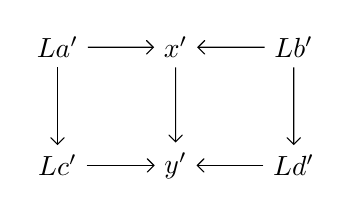
\begin{tikzpicture}[scale=0.75]
    \node (Lc') at (0,0) {$ Lc' $};
    \node (y') at (2,0) {$ y' $};
    \node (Ld') at (4,0) {$ Ld' $};
    \node (La') at (0,2) {$ La' $};
    \node (x') at (2,2) {$ x' $};
    \node (Lb') at (4,2) {$ Lb' $};
    %
    \draw [cd] 
    (La') edge[] (x')
    (Lb') edge[] (x')
    (Lc') edge[] (y')
    (Ld') edge[] (y')
    (La') edge[] (Lc')
    (x') edge[] (y')
    (Lb') edge[] (Ld');
  \end{tikzpicture}
\end{center}

that has a pushout complement. This data induces a
derived rule that appears on the bottom face of
the diagram
%\begin{equation} \label{eq:str_csp_pushout3}
\[  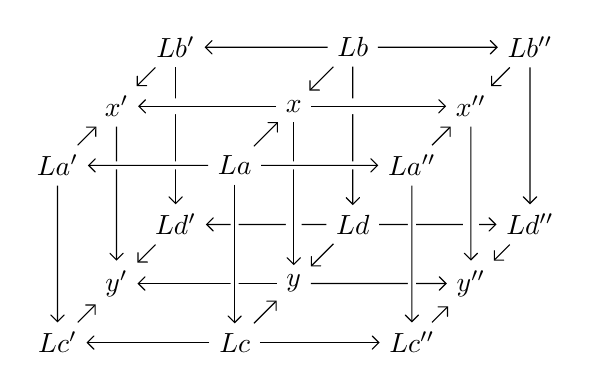
\begin{tikzpicture}[
    scale=0.75,
    baseline=(current  bounding  box.center)]
    \node (La') at (-3,3) {$ La' $};
    \node (x')  at (-2,4) {$ x' $};
    \node (Lb') at (-1,5) {$ Lb' $};
    % 
    \node (Lc') at (-3,0) {$ Lc' $};
    \node (y')  at (-2,1) {$ y' $};
    \node (Ld') at (-1,2) {$ Ld' $};
    %
    \node (La) at (0,3) {$ La $};
    \node (x)  at (1,4) {$ x $};
    \node (Lb) at (2,5) {$ Lb $};
    %
    \node (Lc) at (0,0) {$ Lc $};
    \node (y)  at (1,1) {$ y $};
    \node (Ld) at (2,2) {$ Ld $};
    %
    \node (La'') at (3,3) {$ La'' $};
    \node (x'')  at (4,4) {$ x'' $};
    \node (Lb'') at (5,5) {$ Lb'' $};
    % 
    \node (Lc'') at (3,0) {$ Lc'' $};
    \node (y'')  at (4,1) {$ y'' $};
    \node (Ld'') at (5,2) {$ Ld'' $};
    %
    \draw [cd]
    (Lb)   edge[] (Lb')
    (Lb)   edge[] (Lb'') 
    (Lb')  edge[] (Ld')
    (Lb)   edge[] (Ld)
    (Lb'') edge[] (Ld'')
    (Ld)   edge[] (Ld')
    (Ld)   edge[] (Ld''); 
    %
    \draw [white,line width=2mm]
      (x)   -- (x')
      (x)   -- (x'') 
      (x')  -- (y')
      (x)   -- (y)
      (x'') -- (y'')
      (y)   -- (y')
      (y)   -- (y'');
    \draw [cd]
     (x)   edge[] (x')
     (x)   edge[] (x'') 
     (x')  edge[] (y')
     (x)   edge[] (y)
     (x'') edge[] (y'')
     (y)   edge[] (y')
     (y)   edge[] (y''); 
    %
    \draw [white,line width=1mm]
      (La)   -- (La')
      (La)   -- (La'') 
      (La')  -- (Lc')
      (La)   -- (Lc)
      (La'') -- (Lc'')
      (Lc)   -- (Lc')
      (Lc)   -- (Lc'');
    \draw [cd]
     (La)   edge[] (La')
     (La)   edge[] (La'') 
     (La')  edge[] (Lc')
     (La)   edge[] (Lc)
     (La'') edge[] (Lc'')
     (Lc)   edge[] (Lc')
     (Lc)   edge[] (Lc'');  
     % 
   \draw [cd]
   (Lb')  edge[] (x')
   (Lb)   edge[] (x)
   (Lb'') edge[] (x'')
   (La')  edge[] (x')
   (La)   edge[] (x)
   (La'') edge[] (x'')
   (Ld')  edge[] (y')
   (Ld)   edge[] (y)
   (Ld'') edge[] (y'')
   (Lc')  edge[] (y')
   (Lc)   edge[] (y)
   (Lc'') edge[] (y'');
\end{tikzpicture}\]
%\end{equation}
 This
derived rule is still a rule because pushouts in a topos
preserve monos and epis which, because topoi are
balanced, implies that pushouts also preserve
isomorphisms. In short, derived rules are rules.

%% REWRITE RELATION FOR STRUCTURED COSPANS ~~~~~~~~~~~~

\subsection{Rewrite relation}
\label{sec:rewrite-relation}

Now that we are certain that derivation preserves
rewrite rules of structured cospans, we can look
at the rewrite relation. We can try to encode the
rewrite relation as arrows in a category as we did
with the language functor
$ \Lang \from \Gram \to \Cat $ in Section
\ref{sec:RewriteTopoi}, however, this would fail
to capture the added layer of composition coming
from the structured cospans.  Instead, we give the
type $ \Lang \from \StrCspGram \to \DblCat $ to
the language functor for structured cospans. The
codomain, here, is the category of double
categories and their functors. The language
$ \Lang (_L\StrCsp, P) $, then, is a double
category with structured cospans as horizontal
arrows and certain rewrite rules as
squares. Before defining $ \Lang $ precisely, we
sketch a simple example to help visualize the
language for a structured cospan grammar.

\begin{example}
  Starting with the discrete graph geometric morphism,
  \[
    \adjunction{\RGraph}{L}{R}{\Set}
  \]
  for which $ _L \StrCsp $ is the category of open graphs,
  consider a grammar $ P $ comprising only Rule
  \ref{eq:single_rule_grammar_1}. Then
  $ \Lang (_L\StrCsp,P) $ is the double category whose
  horizontal arrows are open graphs and the existence of a
  square means that the bottom open graph can be obtained by
  removing loops from the top.  For instance,
  $ \Lang (_L\StrCsp,P) $ contains the square
  \begin{center}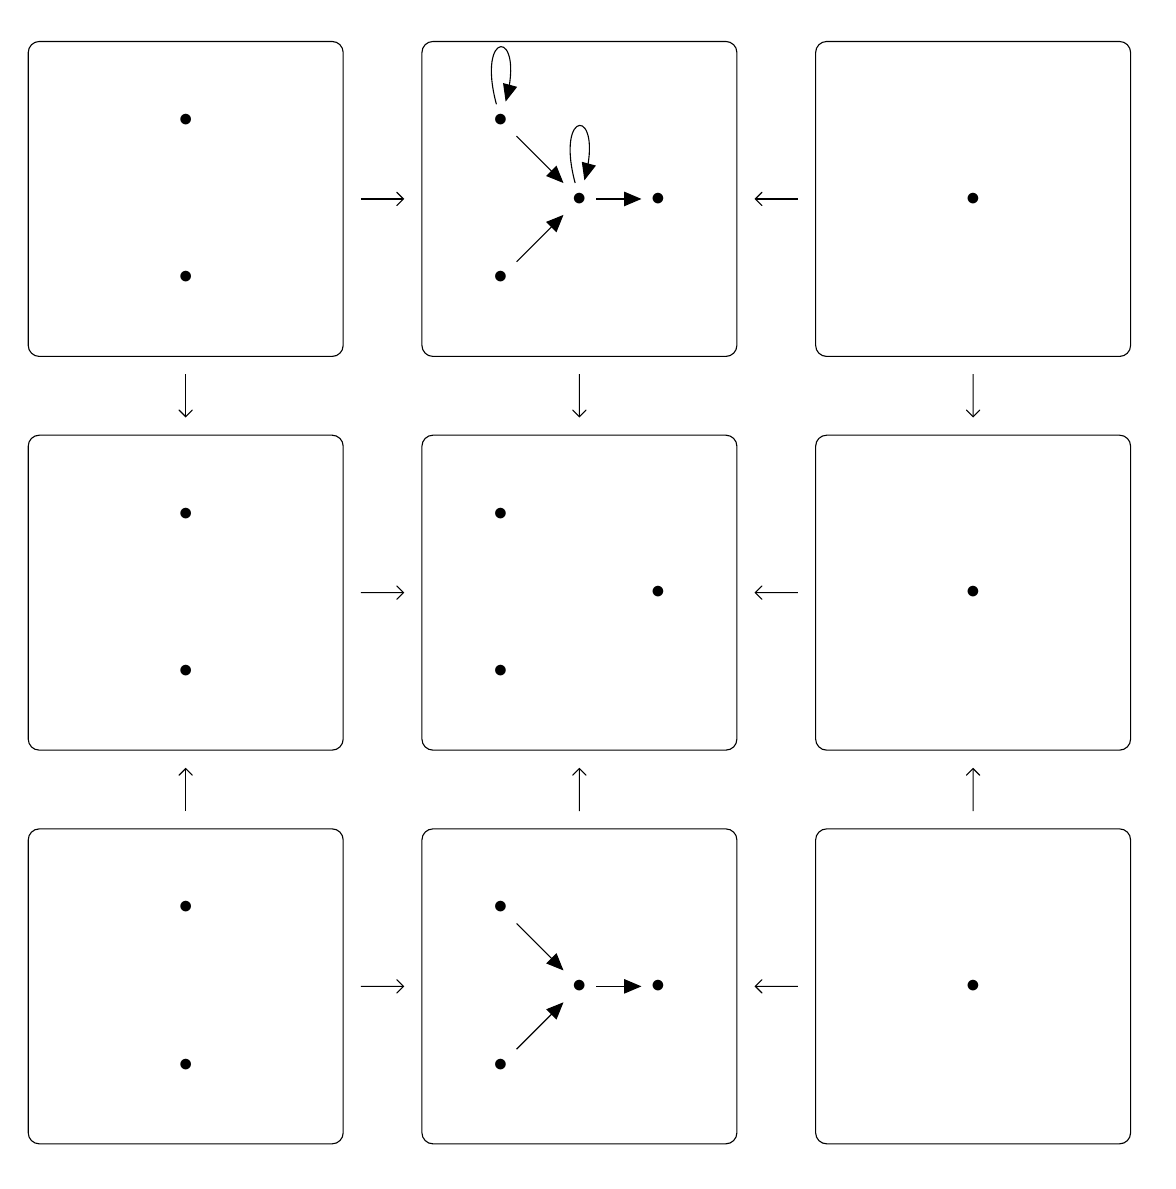
\begin{tikzpicture}
    \begin{scope}[shift={(0,0)}] % up left
      \node (a) at (0,-1) {$ \bullet $};
      \node (b) at (0,1) {$ \bullet $};
      %
      \draw [rounded corners] (-2,-2) rectangle (2,2);
      \node (00r) at (2.1,0) {};
      \node (00b) at (0,-2.1) {};  
    \end{scope}
    %
    \begin{scope}[shift={(5,0)}] % up mid
      \node (a) at (-1,-1) {$ \bullet $};
      \node (b) at (-1,1) {$ \bullet $};
      \node (c) at (0,0) {$ \bullet $};
      \node (d) at (1,0) {$ \bullet $};
      %
      \draw [graph]
        (b) edge[loop above] (b)
        (c) edge[loop above] (c)
        (a) edge[] (c)
        (b) edge[] (c)
        (c) edge[] (d); 
      %  
      \draw [rounded corners] (-2,-2) rectangle (2,2);
      \node (01l) at (-2.1,0) {};
      \node (01r) at (2.1,0)  {};
      \node (01b) at (0,-2.1) {};  
    \end{scope}
    %
    \begin{scope}[shift={(10,0)}] % up right
      \node () at (0,0) {$ \bullet $};
      %
      \draw [rounded corners] (-2,-2) rectangle (2,2);
      \node (02l) at (-2.1,0) {};
      \node (02b) at (0,-2.1) {};
    \end{scope}
    % ~~~~~~~~~~~~~~~~~~~~~~~~~~~~~
    \begin{scope}[shift={(0,-5)}] % mid left
      \node () at (0,-1) {$ \bullet $};
      \node () at (0,1) {$ \bullet $};
      %
      \draw [rounded corners] (-2,-2) rectangle (2,2);
      \node (10t) at (0,2.1)   {};
      \node (10r) at (2.1,0) {};
      \node (10b) at (0,-2.1)  {};  
    \end{scope}
    %
    \begin{scope}[shift={(5,-5)}] % mid mid
      \node (a) at (-1,-1) {$ \bullet $};
      \node (b) at (-1,1) {$ \bullet $};
      \node (d) at (1,0) {$ \bullet $};
      %
      \draw [rounded corners] (-2,-2) rectangle (2,2);
      \node (11l) at (-2.1,0) {};
      \node (11r) at (2.1,0)  {};
      \node (11t) at (0,2.1)  {};
      \node (11b) at (0,-2.1) {};  
    \end{scope}
    %
    \begin{scope}[shift={(10,-5)}] % mid right
      \node () at (0,0) {$ \bullet $};
      %
      \draw [rounded corners] (-2,-2) rectangle (2,2);
      \node (12l) at (-2.1,0) {};
      \node (12t) at (0,2.1)    {};  
      \node (12b) at (0,-2.1)   {};
    \end{scope}
    % ~~~~~~~~~~~~~~~~~~~~~
    \begin{scope}[shift={(0,-10)}] % down left
      \node () at (0,-1) {$ \bullet $};
      \node () at (0,1) {$ \bullet $};
      %
      \draw [rounded corners] (-2,-2) rectangle (2,2);
      \node (20t) at (0,2.1)   {};
      \node (20r) at (2.1,0) {};
      \node (20b) at (0,-2.1)  {};  
    \end{scope}
    %
    \begin{scope}[shift={(5,-10)}] % down mid
      \node (a) at (-1,-1) {$ \bullet $};
      \node (b) at (-1,1) {$ \bullet $};
      \node (c) at (0,0) {$ \bullet $};
      \node (d) at (1,0) {$ \bullet $};
      %
      \draw [graph]
        (a) edge[] (c)
        (b) edge[] (c)
        (c) edge[] (d); 
      %
      \draw [rounded corners] (-2,-2) rectangle (2,2);
      \node (21l) at (-2.1,0) {};
      \node (21r) at (2.1,0)  {};
      \node (21t) at (0,2.1)  {};
      \node (21b) at (0,-2.1) {};  
    \end{scope}
    %
    \begin{scope}[shift={(10,-10)}] % down right
      \node () at (0,0) {$ \bullet $};
      %
      \draw [rounded corners] (-2,-2) rectangle (2,2);
      \node (22l) at (-2.1,0) {};
      \node (22r) at (2.1,0)  {};
      \node (22t) at (0,2.1)  {};
      \node (22b) at (0,-2.1) {};
    \end{scope}
    % ~~~~~~~~~~~~~~~~~~~
    \path[cd]
      (00r) edge (01l)
      (02l) edge (01r)
      (10r) edge (11l)
      (12l) edge (11r)
      (20r) edge (21l)
      (22l) edge (21r)
      (00b) edge (10t)
      (20t) edge (10b)
      (01b) edge (11t)
      (21t) edge (11b)
      (02b) edge (12t)
      (22t) edge (12b);
    \end{tikzpicture}\end{center}
\end{example}

To give a rigorous definition of $ \Lang $, we
first need to define the double category in which
$ \Lang ( _L\StrCsp,P ) $ is generated.

\begin{definition}\label{df:L_SSStrCsp}
  Fix a geometric morphism $L\dashv R \from \X \to
  \A$. There is a double category $_L\SSStrCsp$ whose
  objects are those from $\A$, whose vertical arrows are
  spans with invertible legs in $\A$, whose horizontal
  arrows are $L$-structured cospans, and whose squares
  are $L$-structured cospan rewrite rules.    
\end{definition}

Showing that $_L\SSStrCsp$ is a double category
largely involves checking the requisite list of
axioms. The non-trivial part of this is showing
the interchange law which has been shown in
previous work \parencite[Lem.~4.2,
Lem.~4.3]{CicCour_SpCspTopos}. We should note that
$ _L\SSStrCsp $ is actually a symmetric monoidal
double category via pointwise addition
\parencite[Lem.~4.4]{CicCour_SpCspTopos} (this uses the
fact that $ L $ preserves coproducts), however,
this structure plays no role in this work, so we
do not mention it again.

The following theorem gives the language
functor construction.

\begin{theorem}
  \label{thm:StrCsp_Lang_functorial}
  Let $ L \dashv R \from \X \to \A $ and
  $ L' \dashv R' \from \X' \to \A' $ be geometric
  morphisms. Let $ (_L\StrCsp,P) $ and
  $ ( _{L'}\StrCsp,P' ) $ be structured cospan
  grammars. Let $ dP $ be the set of all
  structured cospan rewrite rules derived from the
  rules in $ P $. Define a relation
  $ \dderiv{}{} $ on $ L $-structured cospans by
  setting
  $$ \dderiv{( La' \to x' \gets Lb' )}{( La'' \to x''
    \gets Lb'' )} $$ if and only if $ dP $ contains a rule
  \begin{center}
  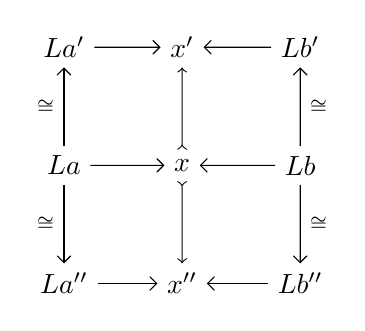
\begin{tikzpicture}[scale=0.75]
    \node (La'') at (0,0) {$ La'' $};
    \node (x'') at (2,0) {$ x'' $};
    \node (Lb'') at (4,0) {$ Lb'' $};
    \node (La) at (0,2) {$ La $};
    \node (x) at (2,2) {$ x $};
    \node (Lb) at (4,2) {$ Lb $};
    \node (La') at (0,4) {$ La' $};
    \node (x') at (2,4) {$ x' $};
    \node (Lb') at (4,4) {$ Lb' $};
    %
    \draw [cd] 
    (La) edge[] (x)
    (Lb) edge[] (x)
    (La') edge[] (x')
    (Lb') edge[] (x')
    (La'') edge[] (x'')
    (Lb'') edge[] (x'')
    %
    (La) edge[] node[left]{$\cong$} (La') 
    (La) edge[] node[left]{$\cong$} (La'')
    (Lb) edge[] node[right]{$\cong$} (Lb')
    (Lb) edge[] node[right]{$\cong$} (Lb'');
    \draw [>->]
    (x) edge (x')
    (x) edge (x'');
  \end{tikzpicture}
\end{center}

  
  There exists a double category
  $ \Lang (_L\StrCsp , P) $ whose objects are
  those of $ \A $, vertical arrows are spans with
  invertible legs in $ \A $, horizontal arrows are
  $ L $-structured cospans, and
  squares are generated by the rules in $ dP $.

  Given a morphism of structured cospan grammars
  $$ (F,G) \from (_L \StrCsp, P) \to ({_L'}\StrCsp , P'), $$
  there is a morphism of double categories
  $$ \Lang (F,G) \from \Lang (_L \StrCsp, P) \to \Lang (_L'
  \StrCsp, P) $$ defined by $ a \mapsto Fa $ on objects and
  extended from
  $ (\dderiv{x}{y}) \mapsto ( \dderiv{Fx}{Fy} ) $ on
  arrows.

  We have, thus, defined a functor
  $ \Lang \from \StrCspGram \to \DblCat $.
\end{theorem}

\begin{proof}
  Define $\Lang (_L\StrCsp,P)$ to be the
  sub-double-category of $_L\SSStrCsp$ generated
  by the squares in $dP$.
  
  Given a morphism of structured cospan grammars
  $$(F,G) \from (_L\StrCsp,P) \to (_{L'}\StrCsp,P'),$$ we
  can define a double functor by extending the definition of
  $F$ on the generating squares. It is certain that
  $\Lang (F,G)$ sends a generating square to a generating
  square because $F$ preserves rules and, because $F$ is
  finitely cocontinuous, preserves derived rules too.  Hence
  $\Lang (F,G)$ sends a generating square in
  $\Lang (_{L}\StrCsp,P)$ to a generating square in
  $\Lang (_{L'}\StrCsp,P')$.
\end{proof}

By construction, $ \Lang $ soundly
encodes the rewrite relation into the squares of a
double category.

\begin{corollary}
  \label{thm:StrCspLang_Encodes_RewrRel}
  Let $ \deriv{}{} $ be the reflexive and
  transitive closure of $ \dderiv{}{} $.  If
  $$ \deriv{\left(\spn{La'}{x'}{Lb'}\right)}{\left(\spn{La''}{x''}{Lb''}\right)}, $$ then there is a square
  \begin{center}
  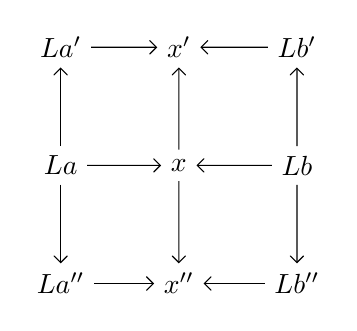
\begin{tikzpicture}[scale=0.75]
    \node (La') at (0,0) {$ La'' $};
    \node (x') at (2,0) {$ x'' $};
    \node (Lb') at (4,0) {$ Lb'' $};
    \node (Lc) at (0,2) {$ La $};
    \node (y) at (2,2) {$ x $};
    \node (Ld) at (4,2) {$ Lb $};
    \node (La) at (0,4) {$ La' $};
    \node (x) at (2,4) {$ x' $};
    \node (Lb) at (4,4) {$ Lb' $};
    \draw [cd]
    (La) edge[] (x)
    (Lb) edge[] (x)
    (La') edge[] (x')
    (Lb') edge[] (x')
    (Lc) edge[] (y)
    (Ld) edge[] (y)
    (Lc) edge[] (La)
    (Lc) edge[] (La')
    (y) edge[] (x)
    (y) edge[] (x')
    (Ld) edge[] (Lb)
    (Ld) edge[] (Lb');
  \end{tikzpicture}
\end{center}
 in
  $ \Lang ({}_L\StrCsp, P) $
\end{corollary}

When rewriting in topoi, we witnessed an
equivalence between the rewrite relation and
language (Theorem
\ref{thm:Lang_from_Gram_to_Cat}). When rewriting
structured cospans, however, we do not expect such
an equivalence for structured cospans because the
rewrite relation $ \deriv{}{} $ only encompasses
the compositionality of the rules, whereas the
language $ \Lang (_L\StrCsp,P) $ captures the
compositionality of both the rules and structured
cospans. Because of this additional compositional
structure, we argue that the rewrite relation is
not the morally correct semantics to study in the
case of structured cospans. 

%% =====================================================
\section{Expressiveness of grammars}
\label{sec:gen-result-graph-rewriting}
%% =====================================================

In general, for any rewrite rule
$ \ell \gets k \to r $, there is only one
constraint on the value of $ k $: it must be a
subobject of $ \ell $ and $ r $.  But requiring
that $ k $ also be discrete can simplify
any analysis involving that rule. This leads us
question whether we can learn about a grammar
$ ( \T,P ) $ by instead studying the grammar
$ ( \T, \flat P ) $, where $ \flat P $ is obtained
by discretizing the apexes of every rule in $ P
$. In this section we explain the $ \flat $
notation and make precise the concept of
discreteness before giving the main result of this
section which states that $ ( \T,P ) $ and
$ ( \T, P_\flat  ) $ have the same rewrite relation
under certain conditions.  This result generalizes
a characterization of discrete graph grammars
given by Ehrig,
et.~al. \parencite[Prop.~3.3]{Ehrig_GraphGram}.

Experts in topos theory know that discreteness
comes from the flat modality on a local
topos. However, we avoid the lengthy detour
required to unpack the meaning of ``the flat
modality on a local topos'' because it does not
benefit our story (curious readers can find this
information elsewhere
\parencite[Ch.~3.6]{Johnstone_Sketches}). Instead, we
offer a more direct, if less subtle, approach by
defining a discrete comonad in a way to fit
our needs.

\begin{definition}[Discrete comonad]
  \label{def:discrete-comonad}
  A comonad on a topos is called \df{discrete} if its counit
  is monic. We use $ \flat $ to denote a discrete comonad.
\end{definition}

We can interpret a discrete comonad as returning
largest interface $ \flat x $ supported by a
system $ x $. If $ x $ is a graph, then $ \flat x
$ is the discrete graph underlying $ x $.  Here is
a brief example illustrating how the discrete graph
adjunction we have made such use of gives rise to
$ \flat $. 

\begin{example}
  Consider the geometric
  morphism $$\adjunction{\Graph}{L}{R}{\Set}$$
  defined by setting $ La $ to be the discrete
  graph on $ a $ and $ Rx $ to be the set of nodes
  in $ x $.  This adjunction induces the comonad
  $ \flat \bydef LR $ on $ \Graph $.  Applying
  $ LR $ to a graph $ x $ returns the discrete
  graph underlying $ x $, for instance
  \[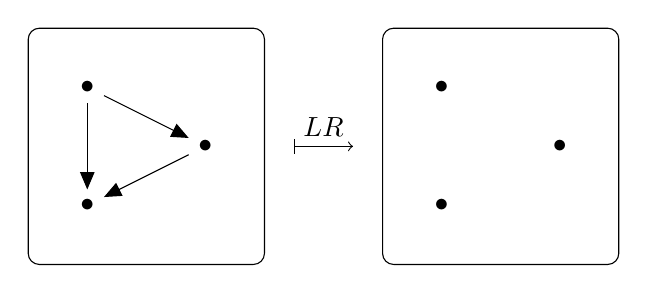
\begin{tikzpicture}[scale=0.75]
    \begin{scope}
      \node (a) at (0,2) {$ \bullet $};
      \node (b) at (2,1) {$ \bullet $};
      \node (c) at (0,0) {$ \bullet $};
      %
      \draw [graph] 
        (a) edge[] (b)
        (a) edge[] (c)
        (b) edge[] (c);
      %
      \draw [rounded corners] (-1,-1) rectangle (3,3);
    \end{scope}
    %
    \begin{scope}[shift={(6,0)}]
      \node (a) at (0,2) {$ \bullet $};
      \node (b) at (2,1) {$ \bullet $};
      \node (c) at (0,0) {$ \bullet $};
      %
      \draw [rounded corners] (-1,-1) rectangle (3,3);
    \end{scope}
    %
    \draw [|->] (3.5,1) to node[above]{$ LR $} (4.5,1);
\end{tikzpicture}\] The
  counit $ \epsilon_x \from LRx \to x $ is
  certainly monic as it includes the discrete
  graph $ LRx $ into the graph $ x $, as in
  \[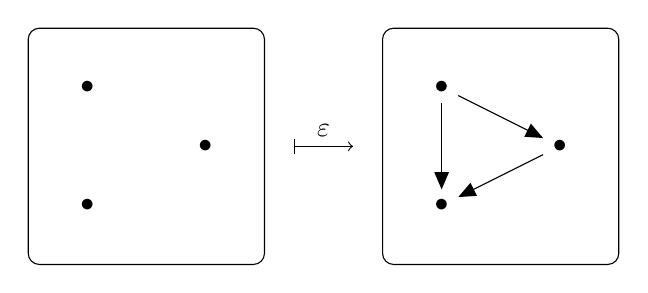
\begin{tikzpicture}[scale=0.75]
    \begin{scope}
      \node (a) at (0,2) {$ \bullet $};
      \node (b) at (2,1) {$ \bullet $};
      \node (c) at (0,0) {$ \bullet $};
      %
      \draw [rounded corners] (-1,-1) rectangle (3,3);
    \end{scope}
    %
    \begin{scope}[shift={(6,0)}]
      \node (a) at (0,2) {$ \bullet $};
      \node (b) at (2,1) {$ \bullet $};
      \node (c) at (0,0) {$ \bullet $};
      %
      \draw [graph] 
        (a) edge[] (b)
        (a) edge[] (c)
        (b) edge[] (c);
      %
      \draw [rounded corners] (-1,-1) rectangle (3,3);
    \end{scope}
    %
    \draw [|->]
      (3.5,1) to node[above]{$ \epsilon $} (4.5,1);
\end{tikzpicture}\]
\end{example}

Discrete comonads provide a tool to control the
form of a grammar by replacing every rule
$ \ell \gets k \to r $ with
$ \ell \gets \flat k \to r $.

\begin{definition}[Discrete grammar]
  \label{def:DiscreteGrammar}
  Let $ \flat \from \T \to \T $ be a discrete
  comonad with counit $ \epsilon $.  Given a
  grammar $ ( \T , P ) $, define $ P_\flat $ as
  the set containing
  \[ \ell \gets k \xgets{\epsilon} \flat k \xto{\epsilon} k \to r \]
  for each rule $ \ell \gets k \to r $ in $ P $. We call $
  ( \T , P_\flat ) $ the \df{discrete grammar} underlying $
  ( \T, P ) $.
\end{definition}

The main result of this section, Theorem
\ref{thm:production-same-rewrite-relation-as-discrete},
says that the grammars $ ( \T,P ) $ and
$ ( \T,P_\flat ) $ have the same rewrite relation
when, for each rule $ \spn{\ell}{k}{r} $ in $ P $,
the subobject lattice $ \Sub(k) $ has all meets. A
reasonable concern is that requiring $ \Sub(k) $
to have all meets is overly restrictive but, in
fact, a fairly large class of grammars has this
property. For instance, this class includes any grammar
built on a presheaf category.  This is especially
pertinent because many systems can be formalized
using labeled graphs, which are presheaves. The
ZX-calculus \parencite{ZX} serves as one example.

\begin{proposition}
  \label{thm:subob-arbitrary-meets}
  Fix an object $k$ of a topos $ \T $.  The subobject
  lattice $ \Sub (k) $ has arbitrary meets when the
  over-category $ T \downarrow k $ has either all products or all coproducts.
\end{proposition}

\begin{proof}
  Because $ T \downarrow t $ is a topos, it has
  equalizers. Thus giving it all products ensures the
  existence of all limits, hence meets.

  In general, a lattice with arbitrary joins also has
  arbitrary meets: define the meet of a subset to be
  the join of all its lower bounds. Because any join in
  $ \Sub (k) $ is a coproduct in $ T \downarrow k $,
  assuming all coproducts provides all joins and, therefore,
  all meets.  
\end{proof}

\begin{corollary}
  Any subobject lattice in a presheaf categories has
  arbitrary meets.  
\end{corollary}

\begin{proof}
  An over-category of presheaves is again a presheaf
  category, hence has all coproducts.  
\end{proof}

At last, we reach our main result of this section.
This result mirrors Chomsky's hierarchy of
grammars \parencite{Chomsky} and the classification of
graph grammars \parencite[Prop.~3.3]{Ehrig_GraphGram}.

\begin{theorem}
  \label{thm:production-same-rewrite-relation-as-discrete}  
  Let $ \T $ be a topos, $ \flat \from \T \to \T $
  be a discrete comonad, and $ ( \T , P ) $ be a
  grammar such that, for every rule
  $ \ell \gets k \to r $ in $ P $, the subobject
  lattice $ \Sub (k) $ has all meets. The rewrite
  relation for $ ( \T , P ) $ equals the rewrite
  relation for its underlying discrete grammar
  $ ( \T,P_\flat ) $.
\end{theorem}

\begin{proof}
  Suppose that $ ( \T,P ) $ induces
  $ \dderiv{g}{h} $. That means there exists a
  rule $ \spn{\ell}{k}{r} $ in $ P $ and a
  derivation \begin{equation} \label{eq:prod-rewrite-1}
  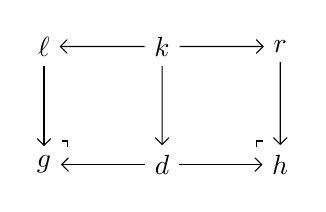
\begin{tikzpicture}[
    scale=0.75,
    baseline=(current  bounding  box.center)]
    \node (1t) at (0,2) {$ \ell $};
    \node (2t) at (2,2) {$ k $};
    \node (3t) at (4,2) {$ r $};
    \node (1b) at (0,0) {$ g $};
    \node (2b) at (2,0) {$ d $};
    \node (3b) at (4,0) {$ h $};
    \draw [cd]
      (2t) edge (1t)
      (2t) edge (3t)
      (2b) edge (1b)
      (2b) edge (3b)
      (1t) edge (1b)
      (2t) edge (2b)
      (3t) edge (3b);
      %
      \draw (0.3,0.4) -- (0.4,0.4) -- (0.4,0.3);
      \draw (3.7,0.4) -- (3.6,0.4) -- (3.6,0.3);
    \end{tikzpicture}
  \end{equation}
  We can achieve that same derivation using rules
  in $ P_\flat $, which requires that we build a
  pushout complement $ w $ of the diagram
  \begin{center}\begin{tikzpicture}
      \node (k) at (0,2) {$ k $};
      \node (bk) at (2,2) {$ \flat k $};
      \node (d) at (0,0) {$ d $};
      %
      \draw [cd]
        (bk) edge[] node[above]{$ \epsilon $} (k)
        (k) edge[] (d); 
  \end{tikzpicture}\end{center} Because
  $ \Sub ( k )$ has all meets, we can define
  $ w \coloneqq \bigwedge \{ z \colon z \vee k = d
  \} \vee \flat k$ which comes with inclusions
  $ \flat k \to w $ and $ w \to d $.  Note that
  $ w \vee k = d $ and $ w \wedge k = \flat k
  $. It follows that
  \[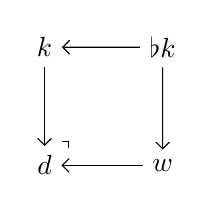
\begin{tikzpicture}[scale=0.75]
      \node (k) at (0,2) {$ k $};
      \node (bk) at (2,2) {$ \flat k $};
      \node (d) at (0,0) {$ d $};
      \node (w) at (2,0) {$ w $};
      %
      \draw [cd] 
      (bk) edge[] (k)
      (bk) edge[] (w)
      (k) edge[] (d)
      (w) edge[] (d);
      %
      \draw (0.3,0.4) -- (0.4,0.4) -- (0.4,0.3);
  \end{tikzpicture}\] is a
  pushout with which we get a derivation
  %
  \begin{equation} \label{eq:prod-rewrite-2}
    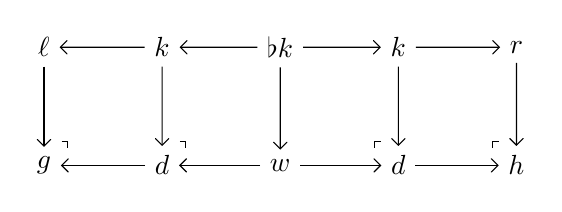
\begin{tikzpicture}[
      scale=0.75,
      baseline=(current  bounding  box.center)]
    \node (01) at (0,2) {$ \ell $};
    \node (11) at (2,2) {$ k $};
    \node (21) at (4,2) {$ \flat k $};
    \node (31) at (6,2) {$ k $};
    \node (41) at (8,2) {$ r $};
    \node (00) at (0,0) {$ g $};
    \node (10) at (2,0) {$ d $};
    \node (20) at (4,0) {$ w $};
    \node (30) at (6,0) {$ d $};
    \node (40) at (8,0) {$ h $};
    %
    \draw [cd] (11) to node [] {\scriptsize{$  $}} (01);
    \draw [cd] (21) to node [] {\scriptsize{$  $}} (11);
    \draw [cd] (21) to node [] {\scriptsize{$  $}} (31);
    \draw [cd] (31) to node [] {\scriptsize{$  $}} (41);
    \draw [cd] (10) to node [] {\scriptsize{$  $}} (00);
    \draw [cd] (20) to node [] {\scriptsize{$  $}} (10);
    \draw [cd] (20) to node [] {\scriptsize{$  $}} (30);
    \draw [cd] (30) to node [] {\scriptsize{$  $}} (40);
    \draw [cd] (01) to node [] {\scriptsize{$  $}} (00);
    \draw [cd] (11) to node [] {\scriptsize{$  $}} (10);
    \draw [cd] (21) to node [] {\scriptsize{$  $}} (20);
    \draw [cd] (31) to node [] {\scriptsize{$  $}} (30);
    \draw [cd] (41) to node [] {\scriptsize{$  $}} (40);
    %
    \draw (0.3,0.4) -- (0.4,0.4) -- (0.4,0.3);
    \draw (2.3,0.4) -- (2.4,0.4) -- (2.4,0.3);
    \draw (5.7,0.4) -- (5.6,0.4) -- (5.6,0.3);
    \draw (7.7,0.4) -- (7.6,0.4) -- (7.6,0.3);
  \end{tikzpicture}\end{equation} with
  respect to $ P_\flat $.  Therefore,
  $ \dderiv{g}{h} $ via $ P $ in Diagram
  \eqref{eq:prod-rewrite-1} implies that
  $ \deriv{g}{h} $ via $ P_\flat $ as shown in
  Diagram \eqref{eq:prod-rewrite-2}.

  For the other direction, suppose $ P_\flat $
  induces $ \dderiv{g}{h} $ via a derivation
  \begin{equation}
  \label{eq:prod-rewrite-3}
  \begin{tikzpicture}
    \node (1t) at (0,2) {$ \ell $};
    \node (2t) at (2,2) {$ \flat k $};
    \node (3t) at (4,2) {$ r $};
    \node (1b) at (0,0) {$ g $};
    \node (2b) at (2,0) {$ d $};
    \node (3b) at (4,0) {$ h $};
    \draw [cd]
      (2t) edge                          (1t)
      (2t) edge                          (3t)
      (2b) edge node[below]{$ \psi $}    (1b)
      (2b) edge                          (3b)
      (1t) edge node[left]{$ m $}        (1b)
      (2t) edge node[left]{$ \theta $}   (2b)
      (3t) edge node[right]{$ m' $}      (3b);
      %
      \draw (0.3,0.4) -- (0.4,0.4) -- (0.4,0.3);
      \draw (3.7,0.4) -- (3.6,0.4) -- (3.6,0.3);
  \end{tikzpicture}
\end{equation} By
  construction, the rule
  $ \spn{\ell}{\flat k}{r} $ in $ P_\flat $ was
  induced by some rule
  \begin{equation}\label{eq:expressivityProof10}
    \ell \xgets{\tau} k \to r
  \end{equation}
  in $ P $. Define $ d' $ to be the pushout of the
  diagram \[\begin{tikzpicture}[scale=0.75]
  \node (flatk) at (0,2) {$ \flat k $};
  \node (k)     at (2,2) {$ k $};
  \node (d)     at (0,0) {$ d $};
  \node (d')    at (2,0) {$ d' $};
  % 
  \draw [cd] 
   (flatk) edge[] node[above]{$ \epsilon $}       (k)
   (flatk) edge[] node[left]{$ \theta $}          (d)
   (d)     edge[] node[below]{$ \hat{\epsilon} $} (d')
   (k)     edge[] node[right]{$ \hat{\theta} $}   (d');
  % 
  \draw (1.7,0.4) -- (1.6,0.4) -- (1.6,0.3);
\end{tikzpicture}\]
  Given the maps $ \psi \from d \to g $ and
  $ m \tau \from k \to \ell \to g$ from
  \eqref{eq:prod-rewrite-3} and
  \eqref{eq:expressivityProof10}, we invoke the
  universal property of $ d' $ to get a canonical
  map $ d' \to g $. This map fits into the diagram
  \begin{center}\begin{tikzpicture}
  \node (l) at (0,2) {$ \ell $};
  \node (g) at (0,0) {$ g $};
  \node (k) at (2,2) {$ k $};
  \node (d') at (2,0) {$ d' $};
  \node (flatk) at (1,3) {$ \flat k $};
  \node (d) at (1,1) {$ d $};
  \draw [cd] 
    (flatk) edge[] (l)
    (flatk) edge[] node[right]{$ \epsilon $} (k)
    (flatk) edge[] node[left,pos=0.7]{$ \theta $} (d)
    (d) edge[] node[below,pos=0.3]{$ \psi $}     (g)
    (d) edge[] node[below,pos=0.3]{$ \hat{\epsilon} $} (d')
    (l) edge[] node[left]{$ m $} (g)
    (k) edge[] node[right]{$ \hat{\theta} $} (d')
    (d') edge[] (g);
  \draw [white,line width=0.5em] (k) -- (l);
  \draw [cd] (k) to node[above,pos=0.3]{$ \tau $} (l);
  % 
  \draw (0.2,0.6) -- (0.3,0.7) -- (0.3,0.6);
  \draw (1.8,0.6) -- (1.7,0.7) -- (1.7,0.6);
\end{tikzpicture}\end{center} whose back
  faces are pushouts. Using a standard diagram
  chasing argument, we can show that the front
  face is also a pushout.  Similarly, the square
  \begin{center}\begin{tikzpicture}[scale=0.75]
  \node (k) at (0,2) {$ k $};
  \node (r) at (2,2) {$ r $};
  \node (d') at (0,0) {$ d' $};
  \node (h) at (2,0) {$ h $};
  % 
  \draw [cd] 
    (k) edge[] (r)
    (k) edge[] (d')
    (d') edge[] (h)
    (r) edge[] (h);
  % 
  \draw (1.7,0.4) -- (1.6,0.4) -- (1.6,0.3);
\end{tikzpicture}\end{center} is a
  pushout.  Sticking these two pushouts together
  gives the double pushout diagram
  \begin{center}\begin{tikzpicture}[scale=0.75]
  \node (1t) at (0,2) {$ \ell $};
  \node (2t) at (2,2) {$ k $};
  \node (3t) at (4,2) {$ r $};
  \node (1b) at (0,0) {$ g $};
  \node (2b) at (2,0) {$ d' $};
  \node (3b) at (4,0) {$ h $};
  \draw [cd]
    (2t) edge                     (1t)
    (2t) edge                     (3t)
    (2b) edge                     (1b)
    (2b) edge                     (3b)
    (1t) edge node[left]{$ m $}   (1b)
    (2t) edge node[left]{$ \hat{\theta} $}   (2b)
    (3t) edge node[right]{$ m' $} (3b);
  \draw (0.3,0.4) -- (0.4,0.4) -- (0.4,0.3);
  \draw (3.7,0.4) -- (3.6,0.4) -- (3.6,0.3);
\end{tikzpicture}\end{center} proving
  that $ P $ induces $ \dderiv{g}{h} $.
\end{proof}


%% =======================================
%% =======================================

\section{An inductive view of rewriting in a topos}
\label{sec:charRewrRelat}

Before graph rewriting, there was formal language rewriting
and term rewriting. In these cases, there are two ways to
define the rewrite relation.  The first way is called the
\emph{operational method}, which applies a rule by
substituting a sub-term for another term.  The second way is
called the \emph{inductive method}, which constructs the
rewrite relation using generators and closure operations. In
classical graph rewriting, only the operational method
existed, where substitution was achieved with the double
pushout method.  Eventually, Gadducci and Heckel introduced
an inductive method to construct the rewrite relation,
opening the way to analyze graph grammars through structural
induction. In this section, we adapt their ideas to give an
inductive definition of the rewrite relation for a grammar
$ ( \X,P ) $ such that $\X $ fits into a geometric morphism
$L \dashv R \from \X \to \A $ with a monic counit.

In the systems perspective, a grammar $( \X,P )$ can be
thought of as comprising a topos $\X$ of closed systems and
a set of rules $P$ stating how to simplify the closed
systems. An important part of our construction involves
decomposing a closed system $x$ into other systems
$x_1, \dotsc, x_n$ that are somehow connected. Structured
cospans provide a way to form these connections, hence why
we want $\X$ to fit into that geometric morphism. Because
our construction uses structured cospans, we need a way to
represent a closed system. We turn a closed system $x$ into
the structured cospan $L0 \gets x \to L0$ with an empty interface.

The particular decomposition we use are determined by the
grammar. That is, we start with a grammar $( \X,P )$, then
fit $\X$ into a geometric morphism
$L \dashv R \from \X \to \A$ with a monic counit. The
geometric morphism gives a discrete comonad
$\flat \bydef LR$ which allows us to form the discrete
grammar $(\X,P_\flat)$ (see Definition
\ref{def:DiscreteGrammar}). Finally, we form a structured
cospan grammar $ ( _L \StrCsp , \hat{P_\flat} ) $ where
$ \hat{P_\flat} $ contains the rule
\begin{equation} \label{eq:decomposition-square}
  \begin{tikzpicture}[scale=0.75,
    baseline=(current  bounding  box.center)]
    \node (1) at (0,4) {$ L 0 $};
    \node (2) at (2,4) {$ \ell $};
    \node (3) at (4,4) {$ LRk $};
    \node (4) at (0,2) {$ L 0 $};
    \node (5) at (2,2) {$ LRk $};
    \node (6) at (4,2) {$ LRk $};
    \node (7) at (0,0) {$ L 0 $};
    \node (8) at (2,0) {$ r $};
    \node (9) at (4,0) {$ LRk $};
    \draw [cd] (1) to (2);
    \draw [cd] (3) to (2);
    \draw [cd] (4) to (5);
    \draw [cd] (6) to (5);
    \draw [cd] (7) to (8);
    \draw [cd] (9) to (8);
    \draw [cd] (4) to (1);
    \draw [cd] (4) to (7);
    \draw [cd] (5) to (2);
    \draw [cd] (5) to (8);
    \draw [cd] (6) to (3);
    \draw [cd] (6) to (9);
  \end{tikzpicture}
\end{equation}
%  for each rule
$ \spn{\ell}{LRk}{r} $ of $ P_{\flat} $. The language $\Lang
( _L \StrCsp , \hat{P_\flat} )$, then, encodes the rewrite
relation for $( \X,P )$ in its squares which are generated
by the rules in $\hat{P_\flat}$. This generation is what
forms the inductive viewpoint of the rewrite relation. 

Prior to proving what the previous paragraph sketched, we
need the following lemma which formalizes the analogy
between rewriting the disjoint union of systems and
tensoring squares.

\begin{lemma} \label{thm:rewrite-rel-is-additive}
  Let $( \X,P )$ be a grammar with rewrite relation $\deriv{}{}$.
  If $ \deriv{x}{y} $ and $ \deriv{x'}{y'} $, then
  $ \deriv{x+x'}{y+y'} $
\end{lemma}

\begin{proof}
  If the derivation $ \deriv{x}{y} $ comes from a string of
  double pushout diagrams
  \begin{center}\begin{tikzpicture}[scale=0.75]
    \node (1t) at (0,2) {$ \ell_1 $};
    \node (2t) at (2,2) {$ k_1 $};
    \node (3t) at (4,2) {$ r_1 $};
    \node (4t) at (6,2) {$ \ell_2 $};
    \node (5t) at (8,2) {$ k_2 $};
    \node (6t) at (10,2) {$ r_2 $};
%    \node (7t) at (11,2) {$ \ell_n $};
    \node (8t) at (11,2) {$ k_n $};
    \node (9t) at (13,2) {$ r_n $};
    \node (1b) at (0,0) {$ x $};
    \node (2b) at (2,0) {$ d_1 $};
    \node (3b) at (5,0) {$ w_1 $};
    \node (4b) at (8,0) {$ d_2 $};
    \node (5b) at (10,0) {$ w_2 $};
%    \node (6b) at (11,0) {$ w_{n-1} $};
    \node (7b) at (11,0) {$ d_n $};
    \node (8b) at (13,0) {$ y $};
    \draw [cd] (2t) to node [] {\scriptsize{$  $}} (1t);
    \draw [cd] (2t) to node [] {\scriptsize{$  $}} (3t);
    \draw [cd] (5t) to node [] {\scriptsize{$  $}} (4t);
    \draw [cd] (5t) to node [] {\scriptsize{$  $}} (6t);
%    \draw [cd] (8t) to node [] {\scriptsize{$  $}} (7t);
    \draw [cd] (8t) to node [] {\scriptsize{$  $}} (9t);
    \draw [cd] (2b) to node [] {\scriptsize{$  $}} (1b);
    \draw [cd] (2b) to node [] {\scriptsize{$  $}} (3b);
    \draw [cd] (4b) to node [] {\scriptsize{$  $}} (3b);
    \draw [cd] (4b) to node [] {\scriptsize{$  $}} (5b);
%    \draw [cd] (7b) to node [] {\scriptsize{$  $}} (6b);
    \draw [cd] (7b) to node [] {\scriptsize{$  $}} (8b);
    \draw [cd] (1t) to node [] {\scriptsize{$  $}} (1b);
    \draw [cd] (2t) to node [] {\scriptsize{$  $}} (2b);
    \draw [cd] (3t) to node [] {\scriptsize{$  $}} (3b);
    \draw [cd] (4t) to node [] {\scriptsize{$  $}} (3b);
    \draw [cd] (5t) to node [] {\scriptsize{$  $}} (4b);
    \draw [cd] (6t) to node [] {\scriptsize{$  $}} (5b);
 %   \draw [cd] (7t) to node [] {\scriptsize{$  $}} (6b);
    \draw [cd] (8t) to node [] {\scriptsize{$  $}} (7b);
    \draw [cd] (9t) to node [] {\scriptsize{$  $}} (8b);
    \node () at (10.5,1) {$ \dotsm $};
    % 
    \draw (0.3,0.4) -- (0.4,0.4) -- (0.4,0.3);
    \draw (4.7,0.4) -- (4.6,0.4) -- (4.6,0.3);
    \draw (5.3,0.4) -- (5.4,0.4) -- (5.4,0.3);
    \draw (9.7,0.4) -- (9.6,0.4) -- (9.6,0.3);
 %   \draw (11.3,0.4) -- (11.4,0.4) -- (11.4,0.3);
    \draw (12.7,0.4) -- (12.6,0.4) -- (12.6,0.3);
  \end{tikzpicture}\end{center}
%  and the derivation
  $ \deriv{x'}{y'} $ comes from a string of double pushout
  diagrams % 
\begin{center} \begin{tikzpicture}[scale=0.75]
  \node (1t) at (0,2) {$ \ell'_1 $};
  \node (2t) at (2,2) {$ k'_1 $};
  \node (3t) at (4,2) {$ r'_1 $};
  \node (4t) at (6,2) {$ \ell'_2 $};
  \node (5t) at (8,2) {$ k'_2 $};
  \node (6t) at (10,2) {$ r'_2 $};
%  \node (7t) at (11,2) {$ \ell'_m $};
  \node (8t) at (11,2) {$ k'_m $};
  \node (9t) at (13,2) {$ r'_m $};
  \node (1b) at (0,0) {$ x' $};
  \node (2b) at (2,0) {$ d'_1 $};
  \node (3b) at (5,0) {$ w'_1 $};
  \node (4b) at (8,0) {$ d'_2 $};
  \node (5b) at (10,0) {$ w'_2 $};
%  \node (6b) at (11,0) {$ w'_{m-1} $};
  \node (7b) at (11,0) {$ d'_m $};
  \node (8b) at (13,0) {$ y' $};
  \draw [cd] (2t) to node [] {\scriptsize{$  $}} (1t);
  \draw [cd] (2t) to node [] {\scriptsize{$  $}} (3t);
  \draw [cd] (5t) to node [] {\scriptsize{$  $}} (4t);
  \draw [cd] (5t) to node [] {\scriptsize{$  $}} (6t);
%  \draw [cd] (8t) to node [] {\scriptsize{$  $}} (7t);
  \draw [cd] (8t) to node [] {\scriptsize{$  $}} (9t);
  \draw [cd] (2b) to node [] {\scriptsize{$  $}} (1b);
  \draw [cd] (2b) to node [] {\scriptsize{$  $}} (3b);
  \draw [cd] (4b) to node [] {\scriptsize{$  $}} (3b);
  \draw [cd] (4b) to node [] {\scriptsize{$  $}} (5b);
%  \draw [cd] (7b) to node [] {\scriptsize{$  $}} (6b);
  \draw [cd] (7b) to node [] {\scriptsize{$  $}} (8b);
  \draw [cd] (1t) to node [] {\scriptsize{$  $}} (1b);
  \draw [cd] (2t) to node [] {\scriptsize{$  $}} (2b);
  \draw [cd] (3t) to node [] {\scriptsize{$  $}} (3b);
  \draw [cd] (4t) to node [] {\scriptsize{$  $}} (3b);
  \draw [cd] (5t) to node [] {\scriptsize{$  $}} (4b);
  \draw [cd] (6t) to node [] {\scriptsize{$  $}} (5b);
%  \draw [cd] (7t) to node [] {\scriptsize{$  $}} (6b);
  \draw [cd] (8t) to node [] {\scriptsize{$  $}} (7b);
  \draw [cd] (9t) to node [] {\scriptsize{$  $}} (8b);
  \node () at (10.5,1) {$ \dotsm $};
  % 
  \draw (0.3,0.4) -- (0.4,0.4) -- (0.4,0.3);
  \draw (4.7,0.4) -- (4.6,0.4) -- (4.6,0.3);
  \draw (5.3,0.4) -- (5.4,0.4) -- (5.4,0.3);
  \draw (9.7,0.4) -- (9.6,0.4) -- (9.6,0.3);
%  \draw (11.3,0.4) -- (11.4,0.4) -- (11.4,0.3);
  \draw (12.7,0.4) -- (12.6,0.4) -- (12.6,0.3);
\end{tikzpicture} \end{center} realize
  $ \deriv{x+x'}{y+y'} $ by the diagram
  \begin{center} \begin{tikzpicture}[scale=0.75]
  \node (1t) at (0,2) {$ \ell_1 $};
  \node (2t) at (2,2) {$ k_1 $};
  \node (3t) at (4,2) {$ r1 $};
  \node () at (12,1) {$ \cdots $};
  \node () at (4.5,1) {$ \cdots $};
  \node (4t) at (5,2) {$ r_n $};
  \node (5t) at (7,2) {$ \ell'_1 $};
  \node (6t) at (9,2) {$ k'_1 $};
  \node (7t) at (11,2) {$ r'_1 $};
  \node (8t) at (13,2) {$ k'_m $};
  \node (9t) at (15,2) {$ r'_m $};
  % 
  \node (1b) at (0,0) {$ x+x' $};
  \node (2b) at (2,0) {$ d_1+x' $};
  \node (3b) at (4,0) {$ w_1+x' $};
  \node (5b) at (6,0) {$ y+x' $};
  \node (6b) at (9,0) {$ y+d'_1 $};
  \node (7b) at (11,0) {$ y+w'_1 $};
  \node (8b) at (13,0) {$ y+d'_m $};
  \node (9b) at (15,0) {$ y+y' $};
  % 
  \draw [cd]
    (2t) edge[] (1t)
    (2t) edge[] (3t)
    (6t) edge[] (5t)
    (6t) edge[] (7t)
    (8t) edge[] (9t) 
    (2b) edge[] (1b)
    (2b) edge[] (3b)
    (6b) edge[] (5b)
    (6b) edge[] (7b)
    (8b) edge[] (9b) 
    (1t) edge[] (1b)
    (2t) edge[] (2b)
    (3t) edge[] (3b)
    (4t) edge[] (5b)
    (5t) edge[] (5b)
    (6t) edge[] (6b)
    (7t) edge[] (7b)
    (8t) edge[] (8b)
    (9t) edge[] (9b);
    %
    \draw (0.3,0.4) -- (0.4,0.4) -- (0.4,0.3);
    \draw (3.7,0.4) -- (3.6,0.4) -- (3.6,0.3);
    \draw (6.3,0.4) -- (6.4,0.4) -- (6.4,0.3);
    \draw (10.7,0.4) -- (10.6,0.4) -- (10.6,0.3);
    % \draw (11.3,0.4) -- (11.4,0.4) -- (11.4,0.3);
    \draw (14.7,0.4) -- (14.6,0.4) -- (14.6,0.3);
  \end{tikzpicture} \end{center}
\end{proof}

\begin{theorem} \label{thm:inductive-rewriting} Let
  $ ( \X , P ) $ be a grammar with rewrite relation
  $\deriv{}{}$. Suppose that for each rule
  $\ell \gets k \to r$ in $P$, the lattice $ \Sub (k) $ has
  all meets.  Let $ L \dashv R \from \X \to \A $ be a
  geometric morphism with monic counit. Then
  $ \deriv{g}{h} $ if and only if there is a square
  %
  \begin{center} \begin{tikzpicture}[scale=0.75]
    \node (1t) at (0,4) {$ LR 0 $};
    \node (2t) at (2,4) {$ g $};
    \node (3t) at (4,4) {$ LR 0 $};
    \node (1m) at (0,2) {$ LR 0 $};
    \node (2m) at (2,2) {$ d $};
    \node (3m) at (4,2) {$ LR 0 $};
    \node (1b) at (0,0) {$ LR 0 $};
    \node (2b) at (2,0) {$ h $};
    \node (3b) at (4,0) {$ LR 0 $};
    % 
    \draw [cd] (1t) to node [] {\scriptsize{$  $}} (2t);
    \draw [cd] (3t) to node [] {\scriptsize{$  $}} (2t);
    \draw [cd] (1m) to node [] {\scriptsize{$  $}} (2m);
    \draw [cd] (3m) to node [] {\scriptsize{$  $}} (2m);
    \draw [cd] (1b) to node [] {\scriptsize{$  $}} (2b);
    \draw [cd] (3b) to node [] {\scriptsize{$  $}} (2b);
    \draw [cd] (1m) to node [] {\scriptsize{$  $}} (1t);
    \draw [cd] (1m) to node [] {\scriptsize{$  $}} (1b);
    \draw [cd] (2m) to node [] {\scriptsize{$  $}} (2t);
    \draw [cd] (2m) to node [] {\scriptsize{$  $}} (2b);
    \draw [cd] (3m) to node [] {\scriptsize{$  $}} (3t);
    \draw [cd] (3m) to node [] {\scriptsize{$  $}} (3b);
  \end{tikzpicture} \end{center}
  % in the double
  category $ \Lang ( _{L}\StrCsp , \hat{P_\flat} ) $.
\end{theorem}

\begin{proof}
  It follows from Theorem
  \ref{thm:production-same-rewrite-relation-as-discrete}
  that both $( \X,P )$ and $( \X,P_{LR} )$ have the same
  rewrite relation.  Thus, we use $\deriv{}{}$ to refer to
  the rewrite relation on the discrete grammar.

  We show sufficiency by inducting on the length of the
  derivation. If $ \deriv{g}{h} $ in a single step, meaning
  that there is a diagram
  %
  \begin{center}\begin{tikzpicture}
    \node (1t) at (0,2) {$ \ell $};
    \node (2t) at (2,2) {$ LRk $};
    \node (3t) at (4,2) {$ r $};
    \node (1b) at (0,0) {$ g $};
    \node (2b) at (2,0) {$ d $};
    \node (3b) at (4,0) {$ h $};
    \draw [cd] (2t) to (1t);
    \draw [cd] (2t) to (3t);
    \draw [cd] (2b) to (1b);
    \draw [cd] (2b) to (3b);
    \draw [cd] (1t) to (1b);
    \draw [cd] (2t) to (2b);
    \draw [cd] (3t) to (3b);
    %
    \draw (0.3,0.4) -- (0.4,0.4) -- (0.4,0.3);
    \draw (3.7,0.4) -- (3.6,0.4) -- (3.6,0.3);
  \end{tikzpicture} \end{center}
  %  then the desired
  square is the horizontal composition of
  %
  \begin{center} \begin{tikzpicture}[scale=0.75]
    \begin{scope}
      \node (1t) at (0,4) {$ L0 $};
      \node (2t) at (2,4) {$ \ell $};
      \node (3t) at (4,4) {$ LRk $};
      \node (4t) at (6,4) {$ d $};
      \node (5t) at (8,4) {$ L0 $};
      \node (1m) at (0,2) {$ L 0 $};
      \node (2m) at (2,2) {$ LRk $};
      \node (3m) at (4,2) {$ LRk $};
      \node (4m) at (6,2) {$ d $};
      \node (5m) at (8,2) {$ L 0 $};
      \node (1b) at (0,0) {$ L 0 $};
      \node (2b) at (2,0) {$ r $};
      \node (3b) at (4,0) {$ LRk $};
      \node (4b) at (6,0) {$ d $};
      \node (5b) at (8,0) {$ L 0 $};
      \draw [cd] (1t) to node [] {\scriptsize{$  $}} (2t);
      \draw [cd] (3t) to node [] {\scriptsize{$  $}} (2t);
      \draw [cd] (3t) to node [] {\scriptsize{$  $}} (4t);
      \draw [cd] (5t) to node [] {\scriptsize{$  $}} (4t);
      \draw [cd] (1m) to node [] {\scriptsize{$  $}} (2m);
      \draw [cd] (3m) to node [] {\scriptsize{$  $}} (2m);
      \draw [cd] (3m) to node [] {\scriptsize{$  $}} (4m);
      \draw [cd] (5m) to node [] {\scriptsize{$  $}} (4m);
      \draw [cd] (1b) to node [] {\scriptsize{$  $}} (2b);
      \draw [cd] (3b) to node [] {\scriptsize{$  $}} (2b);
      \draw [cd] (3b) to node [] {\scriptsize{$  $}} (4b);
      \draw [cd] (5b) to node [] {\scriptsize{$  $}} (4b);
      \draw [cd] (1m) to node [] {\scriptsize{$  $}} (1t);
      \draw [cd] (1m) to node [] {\scriptsize{$  $}} (1b);
      \draw [cd] (2m) to node [] {\scriptsize{$  $}} (2t);
      \draw [cd] (2m) to node [] {\scriptsize{$  $}} (2b);
      \draw [cd] (3m) to node [] {\scriptsize{$  $}} (3t);
      \draw [cd] (3m) to node [] {\scriptsize{$  $}} (3b);
      \draw [cd] (4m) to node [] {\scriptsize{$  $}} (4t);
      \draw [cd] (4m) to node [] {\scriptsize{$  $}} (4b);
      \draw [cd] (5m) to node [] {\scriptsize{$  $}} (5t);
      \draw [cd] (5m) to node [] {\scriptsize{$  $}} (5b);
    \end{scope}
  \end{tikzpicture}\end{center}
%   
  The left square is a generator and the right
  square is the identity on the horizontal arrow
  $ \csp{LRk}{d}{L0} $. The square for a
  derivation $ \dderiv{\deriv{g}{h}}{j} $ is the
  vertical composition of
  %
  \begin{center} \begin{tikzpicture}[scale=0.75]
    \node (1t) at (0,8) {$ L 0 $};
    \node (2t) at (2,8) {$ g $};
    \node (3t) at (4,8) {$ L 0 $};
    \node (1m) at (0,6) {$ L 0 $};
    \node (2m) at (2,6) {$ d $};
    \node (3m) at (4,6) {$ L 0 $};
    \node (1b) at (0,4) {$ L 0 $};
    \node (2b) at (2,4) {$ h $};
    \node (3b) at (4,4) {$ L 0 $};
    \node (1bb) at (0,2) {$ L 0 $};
    \node (2bb) at (2,2) {$ e $};
    \node (3bb) at (4,2) {$ L 0 $};
    \node (1bbb) at (0,0) {$ L 0 $};
    \node (2bbb) at (2,0) {$ j $};
    \node (3bbb) at (4,0) {$ L 0 $};
    \draw [cd] (1t) to node [] {\scriptsize{$  $}} (2t);
    \draw [cd] (3t) to node [] {\scriptsize{$  $}} (2t);
    \draw [cd] (1m) to node [] {\scriptsize{$  $}} (2m);
    \draw [cd] (3m) to node [] {\scriptsize{$  $}} (2m);
    \draw [cd] (1b) to node [] {\scriptsize{$  $}} (2b);
    \draw [cd] (3b) to node [] {\scriptsize{$  $}} (2b);
    \draw [cd] (1m) to node [] {\scriptsize{$  $}} (1t);
    \draw [cd] (1m) to node [] {\scriptsize{$  $}} (1b);
    \draw [cd] (2m) to node [] {\scriptsize{$  $}} (2t);
    \draw [cd] (2m) to node [] {\scriptsize{$  $}} (2b);
    \draw [cd] (3m) to node [] {\scriptsize{$  $}} (3t);
    \draw [cd] (3m) to node [] {\scriptsize{$  $}} (3b);
    \draw [cd] (1bb) to node [] {\scriptsize{$  $}} (2bb);
    \draw [cd] (3bb) to node [] {\scriptsize{$  $}} (2bb);
    \draw [cd] (1bbb) to node [] {\scriptsize{$  $}} (2bbb);
    \draw [cd] (3bbb) to node [] {\scriptsize{$  $}} (2bbb);
    \draw [cd] (1bb) to node [] {\scriptsize{$  $}} (1b);
    \draw [cd] (1bb) to node [] {\scriptsize{$  $}} (1bbb);
    \draw [cd] (2bb) to node [] {\scriptsize{$  $}} (2b);
    \draw [cd] (2bb) to node [] {\scriptsize{$  $}} (2bbb);
    \draw [cd] (3bb) to node [] {\scriptsize{$  $}} (3b);
    \draw [cd] (3bb) to node [] {\scriptsize{$  $}} (3bbb);
  \end{tikzpicture} \end{center}
  %  
  The top square is from $ \deriv{g}{h} $ and the second
  from $ \dderiv{h}{j} $.

  Conversely, proceed by structural induction on the
  generating squares of
  $ \Lang ( _{L}\StrCsp , \hat{P_\flat} ) $.  It suffices to
  show that the rewrite relation is preserved by vertical
  and horizontal composition by generating squares.  Suppose
  we have a square %
  \begin{center}\begin{tikzpicture}[scale=0.75]
    \node (1t) at (0,4) {$ L 0 $};
    \node (2t) at (2,4) {$ w $};
    \node (3t) at (4,4) {$ L 0 $};
    \node (1m) at (0,2) {$ L 0 $};
    \node (2m) at (2,2) {$ x $};
    \node (3m) at (4,2) {$ L 0 $};
    \node (1b) at (0,0) {$ L 0 $};
    \node (2b) at (2,0) {$ y $};
    \node (3b) at (4,0) {$ L 0 $};
    \draw [cd] (2t) to node [] {\scriptsize{$  $}} (1t);
    \draw [cd] (2t) to node [] {\scriptsize{$  $}} (3t);
    \draw [cd] (2m) to node [] {\scriptsize{$  $}} (1m);
    \draw [cd] (2m) to node [] {\scriptsize{$  $}} (3m);
    \draw [cd] (2b) to node [] {\scriptsize{$  $}} (1b);
    \draw [cd] (2b) to node [] {\scriptsize{$  $}} (3b);
    \draw [cd] (1m) to node [] {\scriptsize{$  $}} (1t);
    \draw [cd] (2m) to node [] {\scriptsize{$  $}} (2t);
    \draw [cd] (3m) to node [] {\scriptsize{$  $}} (3t);
    \draw [cd] (1m) to node [] {\scriptsize{$  $}} (1b);
    \draw [cd] (2m) to node [] {\scriptsize{$  $}} (2b);
    \draw [cd] (3m) to node [] {\scriptsize{$  $}} (3b);
  \end{tikzpicture}\end{center}
  corresponding to a derivation $ \deriv{w}{y} $. Composing
  this vertically with a generating square, which must have
  form %
  \begin{center}\begin{tikzpicture}[scale=0.75]
    \node (1t) at (0,4) {$ L 0 $};
    \node (2t) at (2,4) {$ y $};
    \node (3t) at (4,4) {$ L 0 $};
    \node (1m) at (0,2) {$ L 0 $};
    \node (2m) at (2,2) {$ L 0 $};
    \node (3m) at (4,2) {$ L 0 $};
    \node (1b) at (0,0) {$ L 0 $};
    \node (2b) at (2,0) {$ z $};
    \node (3b) at (4,0) {$ L 0 $};
    \draw [cd] (2t) to node [] {\scriptsize{$  $}} (1t);
    \draw [cd] (2t) to node [] {\scriptsize{$  $}} (3t);
    \draw [cd] (2m) to node [] {\scriptsize{$  $}} (1m);
    \draw [cd] (2m) to node [] {\scriptsize{$  $}} (3m);
    \draw [cd] (2b) to node [] {\scriptsize{$  $}} (1b);
    \draw [cd] (2b) to node [] {\scriptsize{$  $}} (3b);
    \draw [cd] (1m) to node [] {\scriptsize{$  $}} (1t);
    \draw [cd] (2m) to node [] {\scriptsize{$  $}} (2t);
    \draw [cd] (3m) to node [] {\scriptsize{$  $}} (3t);
    \draw [cd] (1m) to node [] {\scriptsize{$  $}} (1b);
    \draw [cd] (2m) to node [] {\scriptsize{$  $}} (2b);
    \draw [cd] (3m) to node [] {\scriptsize{$  $}} (3b);
  \end{tikzpicture}\end{center}
  % corresponding
  to a rule $ \spn{y}{L0}{z} $ gives
  %
  \begin{center}\begin{tikzpicture}[scale=0.75]
    \node (1t) at (0,4) {$ L 0 $};
    \node (2t) at (2,4) {$ w $};
    \node (3t) at (4,4) {$ L 0 $};
    \node (1m) at (0,2) {$ L 0 $};
    \node (2m) at (2,2) {$ L 0 $};
    \node (3m) at (4,2) {$ L 0 $};
    \node (1b) at (0,0) {$ L 0 $};
    \node (2b) at (2,0) {$ z $};
    \node (3b) at (4,0) {$ L 0 $};
    \draw [cd] (2t) to node [] {\scriptsize{$  $}} (1t);
    \draw [cd] (2t) to node [] {\scriptsize{$  $}} (3t);
    \draw [cd] (2m) to node [] {\scriptsize{$  $}} (1m);
    \draw [cd] (2m) to node [] {\scriptsize{$  $}} (3m);
    \draw [cd] (2b) to node [] {\scriptsize{$  $}} (1b);
    \draw [cd] (2b) to node [] {\scriptsize{$  $}} (3b);
    \draw [cd] (1m) to node [] {\scriptsize{$  $}} (1t);
    \draw [cd] (2m) to node [] {\scriptsize{$  $}} (2t);
    \draw [cd] (3m) to node [] {\scriptsize{$  $}} (3t);
    \draw [cd] (1m) to node [] {\scriptsize{$  $}} (1b);
    \draw [cd] (2m) to node [] {\scriptsize{$  $}} (2b);
    \draw [cd] (3m) to node [] {\scriptsize{$  $}} (3b);
  \end{tikzpicture}\end{center}
  % which corresponds
  to a derivation $ \dderiv{\deriv{w}{y}}{z} $.  Composing
  horizontally with a generating square
  %
  \begin{center}\begin{tikzpicture}[scale=0.75]
    \node (1t) at (0,4) {$ L 0 $};
    \node (2t) at (2,4) {$ \ell $};
    \node (3t) at (4,4) {$ L 0 $};
    \node (1m) at (0,2) {$ L 0 $};
    \node (2m) at (2,2) {$ LRk $};
    \node (3m) at (4,2) {$ L 0 $};
    \node (1b) at (0,0) {$ L 0 $};
    \node (2b) at (2,0) {$ r $};
    \node (3b) at (4,0) {$ L 0 $};
    \draw [cd] (2t) to node [] {\scriptsize{$  $}} (1t);
    \draw [cd] (2t) to node [] {\scriptsize{$  $}} (3t);
    \draw [cd] (2m) to node [] {\scriptsize{$  $}} (1m);
    \draw [cd] (2m) to node [] {\scriptsize{$  $}} (3m);
    \draw [cd] (2b) to node [] {\scriptsize{$  $}} (1b);
    \draw [cd] (2b) to node [] {\scriptsize{$  $}} (3b);
    \draw [cd] (1m) to node [] {\scriptsize{$  $}} (1t);
    \draw [cd] (2m) to node [] {\scriptsize{$  $}} (2t);
    \draw [cd] (3m) to node [] {\scriptsize{$  $}} (3t);
    \draw [cd] (1m) to node [] {\scriptsize{$  $}} (1b);
    \draw [cd] (2m) to node [] {\scriptsize{$  $}} (2b);
    \draw [cd] (3m) to node [] {\scriptsize{$  $}} (3b);
  \end{tikzpicture}\end{center}
  % corresponding with
  a rule $ \spn{\ell}{LRk}{r} $ results in the square
  %
  \begin{center}\begin{tikzpicture}[scale=0.75]
    \node (1t) at (0,4) {$ L 0 $};
    \node (2t) at (2,4) {$ w + \ell $};
    \node (3t) at (4,4) {$ L 0 $};
    \node (1m) at (0,2) {$ L 0 $};
    \node (2m) at (2,2) {$ x + LRk $};
    \node (3m) at (4,2) {$ L 0 $};
    \node (1b) at (0,0) {$ L 0 $};
    \node (2b) at (2,0) {$ y + r $};
    \node (3b) at (4,0) {$ L 0 $};
    \draw [cd] (2t) to node [] {\scriptsize{$  $}} (1t);
    \draw [cd] (2t) to node [] {\scriptsize{$  $}} (3t);
    \draw [cd] (2m) to node [] {\scriptsize{$  $}} (1m);
    \draw [cd] (2m) to node [] {\scriptsize{$  $}} (3m);
    \draw [cd] (2b) to node [] {\scriptsize{$  $}} (1b);
    \draw [cd] (2b) to node [] {\scriptsize{$  $}} (3b);
    \draw [cd] (1m) to node [] {\scriptsize{$  $}} (1t);
    \draw [cd] (2m) to node [] {\scriptsize{$  $}} (2t);
    \draw [cd] (3m) to node [] {\scriptsize{$  $}} (3t);
    \draw [cd] (1m) to node [] {\scriptsize{$  $}} (1b);
    \draw [cd] (2m) to node [] {\scriptsize{$  $}} (2b);
    \draw [cd] (3m) to node [] {\scriptsize{$  $}} (3b);
  \end{tikzpicture}\end{center}
  % But
  $ \deriv{w+\ell}{y+r} $ as seen in Lemma
  \ref{thm:rewrite-rel-is-additive}.
\end{proof}


\printbibliography
% \bibliographystyle{plain}
% \bibliography{assets/reopn}



\end{document}

